\documentclass[12pt]{article}

\usepackage[a4paper]{geometry} % a package for setting layout and margins for your thesis 
\usepackage[utf8]{inputenc} % standard encoding since 2018 (can be commented out?)
\usepackage[T1]{fontenc} % absolutely critical for *hyphenation* of words with non-ASCII letters.
\usepackage{times} % typeset text in Times Roman instead of Computer Modern (EC)

% babel
\usepackage[estonian, english]{babel}
\usepackage{csquotes}
\addto\captionsestonian{%
  \renewcommand{\refname}{Viidatud kirjandus}%
  \renewcommand{\appendixname}{Lisad}%
}

% viitamine
\usepackage[giveninits=true]{biblatex}
\DefineBibliographyStrings{estonian}{and={ja}}
\addbibresource{bibliography.bib}

% general packages for math
\usepackage{amsmath} 
\usepackage{amsthm}
\usepackage{amssymb}

% print a dot instead of colon in table or figure captions
\usepackage[labelsep=period]{caption}

% packages for building tables and tabulars 
\usepackage{array}
\usepackage{tabu}   % wide lines in tables
\usepackage{xspace} % non-eatable spaces in macros
\usepackage{float}  % float options

% including graphical images and setting the figure directory
\usepackage{graphicx}
\graphicspath{{joonised/}}

% packages for getting clickable links in PDF file
\usepackage[hidelinks]{hyperref}
\usepackage[all]{hypcap}

% statistilised operaatorid
\DeclareMathOperator*{\MEAN}{\mathbf{E}}
\DeclareMathOperator*{\VARIANCE}{\mathbf{D}}
\newcommand{\mean}[1]{\MEAN\left[#1\right]}
\newcommand{\variance}[1]{\VARIANCE\left[#1\right]}
\newcommand{\prob}[1]{\Pr\left[#1\right]}

% kvaliteedimõõtude definitsioonid
\newcommand{\accuracy}{Acc}
\newcommand{\precision}{Prec}
\newcommand{\recall}{Rec}

\begin{document}

% tiitelleht
\thispagestyle{empty}
\begin{center}

\large{
TARTU ÜLIKOOL\\
Loodus- ja täppisteaduste valdkond\\
Arvutiteaduse instituut\\
Informaatika õppekava\\
}

\vspace{25mm}

\Large Mart-Mihkel Aun

\vspace{4mm}

\huge Masinõppe mudelite hindamine väheste märgenditega andmetel

\vspace{20mm}

\Large{Bakalaureusetöö (9 EAP)}

\end{center}

\vspace{2mm}

\begin{flushright}
    {
    \setlength{\extrarowheight}{5pt}
    \begin{tabular}{r l} 
        \sffamily Juhendaja: & \sffamily Sven Laur, DSc. (Tech)  \\
    \end{tabular}
    }
\end{flushright}

\vfill
\centerline{\large Tartu \the\year}


% abstrakt
% eesti keeles
\selectlanguage{estonian}

\noindent\textbf{\large Masinõppe mudelite hindamine väheste märgenditega andmetel}
\vspace*{1ex}
\noindent\textbf{Lühikokkuvõte:}
\noindent
Klassifitseerimisülesandeid lahendavate masinõppe mudelite hindamiseks kasutatakse kvaliteedimõõte nagu õigsus täpsus ja saagis. Need suurused või nende hinnangud avalduvad andmepunktide tegelike klassimärgendite ja meetodi klassifikatsioonide kaudu. Tegelike klassimärgendite leidmiseks peame need manuaalselt üle vaatama. Sageli hinnatakse kvaliteedimõõte üle lõpliku valimi, leitud hinnangud sisaldavad vigu. Antud töö käigus avaldame vajaliku valimi suuruse, et mingi kindlusega ei ületaks hinnangu viga selle lubatud piiri. Lisaks peame valimi puhul õigsuse, täpsuse või saagise hindamiseks definitsiooni põhjal leidma kõikide valimi andmepunktide märgendid. Kui lisaks hinnatavale klassifitseerimismeetodile on olemas teine meetod, saame seda kasutada esimese hindamiseks. Seejuures on võimalik märgendamiseks vajalikku manuaalset tööd vähendada, kui uurime uue meetodi kvaliteedimõõdu arvutamise asemel kui palju on uus meetod vanast parem. Töös uurime tehnikaid, mis aitavad vähendada märgendamist vajavate andmepunktida arvu kahe klassifitseerimismeetodi kvaliteedimõõtude vahede hindamiseks.
\vspace*{1ex}

\noindent\textbf{Võtmesõnad:} masinõpe, klassifitseerimine, tõenäosusteooria, statistika, õigsus, täpsus, saagis
\vspace*{1ex}

\noindent\textbf{CERCS:}P176 Tehisintellekt
\vspace*{3ex}

% inglise keeles
\selectlanguage{english}

\noindent\textbf{\large Evaluating machine learning models on data with few labels}
\vspace*{1ex}
\noindent\textbf{Abstract:}
\noindent
Machine learning models used to solve classification tasks are evaluated using quality measures such as accuracy, precision, and recall. These measures or their estimates are calculated using the class labels of data points and the classifications made by the method on those data points. To find the actual class labels, we must manually review the datapoints. Quality measures are often evaluated using a finite sample, and the obtained estimates contain errors. In this thesis we determine the necessary sample size for the estimates not to exceed a given limit of their error with a certain confidence level. The definition-based method for determining accuracy, precision, or recall over a given sample requires all the data points' labels to be known. If we have a second method alongside the one being evaluated, we can use it to asses the first. In this case, we can reduce the amount of manual work required for labeling by estiamting how much better the new method is compared to the old one. In this thesis we explore techniques which help reduce the number of data points that require labeling for evaluating the quality measures of the two classification methods.
\vspace*{1ex}

\noindent\textbf{Keywords:} machine learning, classification, probability theory, statistics, accruacy, precision, recall
\vspace*{1ex}

\noindent\textbf{CERCS:}P176 Artificial intelligence
\vspace*{1ex}

\selectlanguage{estonian}

% sisukord
\tableofcontents

% töö ise
\section{Sissejuhatus}
Masinõppe mudelite hindamiseks kasutatakse erinevaid viise. Klassifitseerimisülesannete puhul saab ülesannet lahendava masinõppe meetodi headust hinnata kvaliteedimõõtudega. Kolm tihti kasutatud kvaliteedimõõtu on õigsus, täpsus ja saagis. Õigsus, täpsus ja saagis on nulli ja ühe vahelised numbrilised suurused, kus suurem väärtus tähendab paremat mudelit. Nimetatud suurused või nende hinnangud avalduvad mingi hulga andmepunktide tegelike klassimärgendite ja meetodi poolt klassifitseeritud klassimärgendite kaudu. Tegelike klassimärgendite leidmiseks peab need manuaalselt üle vaatama, mis võib paljude andmepunktide puhul muutuda kulukaks. Kvaliteedimõõtude täpsete väärtuste arvutamiseks peaks teadma populatsiooni kõigi andmepunktide märgendeid. Kuna kogu populatsiooni uurimine ei pruugi praktikas olla võimalik, leitakse sageli kvaliteedimõõtudele hinnangud üle lõpliku valimi.

Üle valimi arvutatud suuruste hinnangud ei ühti tavaliselt nende suuruste oodatud väärtusega, ehk üle populatsiooni arvutatud suurustega. Leitud hinnangud sisaldavad valimi juhuslikkuse tõttu vigu. Seega tuleb küsimuse alla kui suur antud viga on ning kui kindel saab olla, et viga ei ole suurem kui võib lubada. Antud töö käigus leitakse kui suurt valimit on vaja (või kui väikest valimit võib võtta), et mingi kindlusega ei ületaks hinnangu viga selle lubatud piiri.

Valimi puhul peab õigsuse, täpsuse või saagise hindamiseks definitsiooni põhjal leidma kõikide valimi andmepunktide märgendid. Ka minimaalse võimaliku valimi puhul võib see olla probleemne. Juhul kui asendada vana mudelit uuega ei pea küsima mis on uue meetodi õigsus, võib ka uurida kas ja kui palju on uue meetodi õigsus suurem vana omast. Selles töös on uuritud tehnikaid, mis aitavad vähendada märgendamist vajavate andmepunktida arvu kahe klassifitseerimismeetodi kvaliteedimõõtude vahede hindamiseks.

Esimese osas on toodud töös kasutatud mõisted ja definitsioonid ning kirjeldatud töö mõistmist abistavad taustteadmised. Töö teises osas on defineeritud klassifitseerimismeetodi kvaliteedimõõdud nende oodatud väärtuste kaudu, kirjeldatud viise nende hindamiseks ning uuritud kui suurt valimit on vaja küllaltki suure kindlusega piisavalt täpse hinnangu leidmiseks. Kolmandas osas uuritakse kuidas hinnata uut klassifitseerimismeetodit võrreldes seda juba olemasolevaga ning selle juures vältida kõikide andmepunktide märgendamist.
\section{Taust}
Masinõppemeetodite tulemuslikkuse mõõtmiseks kasutatakse mitmeid teoreetilisi kvaliteedimõõtusid. Kvaliteedimõõdud on defineeritud läbi nende ooteväärtuste. Praktikas hinnatakse kvaliteedimõõtusid ligikaudselt, arvutades keskmisi väärtusi üle valimi.

\subsection{Lõplikud ja lõpmatud andmekogumid}
Statistilises uuringus nimetatakse uuringu all olevat objekti üldkogumiks ehk populatsiooniks. Populatsioon koosneb andmepunktidest. Andmepunktide kogus on määratletud populatsiooni korral tavaliselt lõplik. Kõikse uuringu korral mõõdetakse kõiki populatsiooni andmepunkte. Kõikne uuring on sageli ülemäära kulukas. Lihtsam on mõõta juhuslikku osahulka populatsiooni andmepunktidest. Mõõdetavate andmepunktide hulka nimetatakse valimiks. Valimi põhjal tehakse järeldusi kogu populatsiooni kohta. Tehtud järeldused võivad valimi juhuslikkuse tõttu sisaldada vigu, kuid sellised vead on tõenäosuslikult hinnatavad~\cite{rakendusstatisika-algkursus}.

Vahel pole populatsioon uuringu tegemise hetkel üheselt fikseeritud või lõplik, nagu näiteks kõik järgmise 24 tunni jooksul kiirabisse pöörduvad inimesed või kõigi Canon 70D fotokaameratega tehtud pildid. Sellisel juhul määrab tulemuse andmeid genereeriv füüsiline protsess ning seda mudeldatakse tihti juhusliku jaotusega. Formaalselt on juhuslik jaotus andmete allikas, millest saame võtta kuitahes palju sõltumatuid andmepunkte. Antud töös vaatame protsesse, millel on lõplik arv väljundväärtusi, see tähendab, et jaotus on diskreetne. Sel juhul fikseerib jaotus iga konkreetse andmepunkti jaoks selle esinemistõenäosuse, millest võimw mõelda kui andmepunkti oodatavat sagedusest valimis, millesse on võetud piisavalt palju andmepunkte jaotusest.

Lõpliku valimi korral saame mingi uuritava omaduse $A$ esinemise tõenäosust defineerida kui suhet omaduse esinemise arvu valimis $n_A$ ning valimi suuruse $n$ vahel
\begin{equation*}
    \prob{A} = \frac{n_A}{n} \enspace.
\end{equation*}
Juhuslikust valimist juhusliku andmepunkti võtmiselt tähendab see tõenäosust, et andmepunkt on omadusega $A$.

Juhuslikku valimit saame moodustada võttes populatsioonist andmepunkte üksteisest sõltumatult ja juhuslikult. Võib juhtuda, et samad populatsiooni andmepunktid sattuvad valimisse mitmekordselt. Saadud valimi puhul eeldame, et kõik selle andmepunktid on sama jaotusega. Tegelikkuses ei pruugi sõltumatuse ja sama jaotuse eeldus olla täidetud. Näiteks Canon 70D fotokaameraga tehtud pildiseeria piltide jaotused on üksteisega korreleeritud, kuna ühest sündmusest tehakse tavaliselt mitu pilti. See-eest üksikute piltide jaotuste puhul võib sageli sõltumatust eeldada. Valimikeskmine on valimi kõikide andmepunktide väärtuste aritmeetiline keskmine
\begin{equation}
    \label{eq:valimikeskmine}
    \bar{x} = \frac{1}{n} \cdot \sum_{i = 1}^{n} x_i \enspace.
\end{equation}
Juhul kui $x_i$ on indikaator valimi $i$-nda andepunkti mingi omaduse kohta, läheneb valimikeskmine $\bar{x}$ tõenäosusele, et juhuslikul objektil on see omadus.

Valimidispersioon on kõigi andmepunktide hälvete ruutude aritmeetiline keskmine
\begin{equation}
    \label{eq:nihkega valimidispersioon}
    s^2 = \frac{1}{n} \cdot \sum_{i = 1}^{n} (x_i - \bar{x})^2 \enspace.
\end{equation}
Dispersioon näitab andmete hajuvust. Valimidispersiooni kaudu saame leida hinnangu valimikeskmise dispersioonile $\frac{s^2}{n}$, millest ruutjuurt nimetatakse standardveaks~\cite{rakendusstatisika-algkursus}. Standardviga näitab valimikeskmise $\bar{x}$ fluktuatsiooni tema oodatud väärtusest, ehk mitut tüvenumbrit hinnangust võime usaldada.

Olgu olemas juhuslik protsess, mis genereerib populatsiooni andmepunkte. Protsessi genereeritud andmepunktid on üksteisest sõltumatud ja sama jaotusega. Jaotuse abil defineeritud potentsiaalselt lõpmatu andmestiku uurimiseks defineeritakse valimiüleste valemite~\eqref{eq:valimikeskmine} ja~\eqref{eq:nihkega valimidispersioon} analoogid, milleks need lõpmata suure valimi korral koonduvad.

Valimikeskmise analoog keskväärtus iseloomustab jaotuse väärtuste paiknevust, mõnikord nimetatakse keskväärtust ka matemaatiliseks ootuseks~\cite{tõenäosusteooria-algkursus}. Diskreetse juhusliku suuruse $X$ keskväärtus on defineeritud summana
\begin{equation}
    \label{eq:keskväärtus}
    \mean{X} = \sum_{i} x_i p_i \enspace,
\end{equation}
kus $x_i$ on suuruse üks võimalik väärtus ning $p_i$ tõenäosus, et $X$ selle väärtuse võtab. Pideva juhusliku suuruse $X$, mille tihedusfunktsioon on $f_X(x)$, keskväärtus on leitav määratud integraalina
\begin{equation*}
    \mean{X} = \int_{-\infty}^{\infty} x \cdot f_X(x) dx \enspace,
\end{equation*}
mitmemõõtmelise juhusliku suuruse korral on selle keskväärtus leitav analoogiliselt, mitmemõõtmelise integraaliga.

Valimidispersiooni analoog dispersioon on juhusliku suuruse hälve ruudu keskväärtus
\begin{equation}
    \label{eq:dispersioon}
    \variance{X}=\mean{(X - \mean{X})^2} = \mean{X^2} - \mean{X}^2 \enspace.
\end{equation}
Ruutjuurt dispersioonist nimetatakse standardhälbeks. Lõpliku populatsiooni korral avalduvad jaotuseülesed valemid~\eqref{eq:keskväärtus} ja~\eqref{eq:dispersioon} neile vastavate valimiüleste valemitena~\eqref{eq:valimikeskmine} ja~\eqref{eq:nihkega valimidispersioon}. Jaotuseülesed valemeid on vaja, et uurida juhuslikkust sisaldavate suuruste oodatud käitumist.

\subsection{Veahinnangud}
\label{section:veahinnangud}
Numbriliselt ülesannete lahendamisel võib täpse lahendi leidmine olla aeganõudev ja kulukas. Ülesande ligikaudne lahendamine võib osutuda otstarbekamaks, näiteks populatsiooni keskväärtuse leidmise asemel võime leida valimikeskmise. Antud näite korral on valimikeskmine ligikaudne hinnang keskväärtusele. Ligikaudsete väärtuste headust saame mõõta kasutades veahinnanguid. Veahinnangud kirjeldavad mingi täpse arvu ja selle arvu lähendi erinevust. Vastuse lähendamisel praktilises olukorras ei pruugi me teade täpset lahendit. See-eest sobivad veahinnangud lähendamismeetodite teoreetiliseks hindamiseks.

Olgu $a$ ligikaudne väärtus arvust $a_0$. Ligikaudse arvu $a$ absoluutseks veaks nimetatakse arvu
\begin{equation*}
    \Delta a = a - a_0 \enspace.
\end{equation*}
Absoluutse vea õigesti mõistmiseks tuleb arvestada lähendatava arvu skaalaga. Arvude puhul, mis ulatuvad mitmetesse tuhandetesse, tähendab absoluutne viga $0{,}5$ väga täpset lähendit. Nulli ja ühe vaheliste arvude puhul mitte. Seevastu saame kasutada hinnangut, mis arvestab arvude skaalaga. Ligikaudse arvu $a$ relatiivseks ehk suhteliseks veaks nimetatakse suurust
\begin{equation*}
    \delta a = \frac{\Delta a}{a_0} = \frac{a - a_0}{a_0} = \frac{a}{a_0} - 1 \enspace.
\end{equation*}
Mõnikord esitatakse relatiivne viga protsentides.

Ligikaudsete lähendite puhul taheme nende veahinnanguid absoluutväärtuselt minimeerimine. Alati ei pruugi see olla võimalik ning peame leppima mingi veaga. Lisaks võib raske olla täielikult veenduda, et leitud lähendi viga on väiksem kui maksimaalne viga, mida võime lubada. See-eest võime uurida kui suure tõenäosusega on saavutatud viga, mis on väiksem lubatud maksimaalsest veast
\begin{equation*}
    \prob{\mid a - a_0 \mid < \varepsilon} = 1 - \alpha \enspace,
\end{equation*}
kus $\varepsilon$ on absoluutse vea absoluutväärtuse ülemine piir, suurust $\alpha$ nimetatakse olulisusnivooks ning vahet $1-\alpha$ usaldusnivooks või kindluseks. Tihti valitakse $\alpha$ väärtuseks $0{,}05$, mõnikord ka $0{,}01$ või isegi $0{,}32$.

Kui juhuslik suurus on vaadeldav paljude sõltumatute juhuslike suuruste summana on alust arvata, et summa on ligikaudu normaaljaotusega~\cite{tõenäosusteooria-algkursus}. Seega kui ligikaudsed väärtused sisaldavad paljude sõltumatute juhuslike veakomponentide summat võime ka vastavate veahinnangute puhul eeldada, et need on normaaljaotusega.

Juhuslik suurus $X$ on normaaljaotusega kui tema tihedusfunktsioon on
\begin{equation*}
    f_X(x) = \frac{1}{\sqrt{2 \pi} \sigma} \cdot \exp{\left( -\frac{(x - \mu)^2}{2\sigma^2} \right)} \enspace,
\end{equation*}
kus jaotuse parameetrid $\mu$ ja $\sigma$ on vastavalt $X$ keskväärtus ja standardhälve. Seda fakti tähistatakse lühidalt $X \sim \mathcal{N}(\mu, \sigma)$. Normaaljaotuse tihedus on sümmeetriline keskväärtuse $\mu$ ümber. Veahinnangute puhul on nende oodatud väärtus null, siis sümmeetrilisuse tõttu on negatiivsed ja positiivsed vead sama tõenäolised. Oluline omadus normaaljaotuse puhul on see, kui suure tõenäosuse katavad standardhälbe täisarvkordsed vahemikud keskväärtuse ümbruses. Vahemik $\mu \pm \sigma$ katab tõenäosuse $68\%$, $\mu \pm 2\sigma$ tõenäosuse $95\%$ ning $\mu \pm 3\sigma$ tõenäosuse $99\%$.

\subsubsection{Summa ja vahe relatiivse vea omadus}
Vahel võib uuritav suurus olla arvutatav mitme ligikaudse suuruse kaudu. Ligikaudsete suuruste vead kanduvad arvutusi tehes tulemustele edasi. Seega uurime tulemuse täpsuse hindamiseks kuidas viga arvutustel edasi kandub. Sealjuures teeme lihtsustava eelduse, et lähendid on normaaljaotusega.

Olgu $x$ ja $y$ ligikaudsed väärtused arvudest $x_0$ ja $y_0$ absoluutsete vigadega vastavalt $\varepsilon_x$ ning $\varepsilon_y$:
\begin{align*}
    x &= x_0 + \varepsilon_x ,\qquad \varepsilon_x \sim \mathcal{N}(0, \sigma_x) \enspace,\\
    y &= y_0 + \varepsilon_y ,\qquad \varepsilon_y \sim \mathcal{N}(0, \sigma_y) \enspace,
\end{align*}
kus vead $\varepsilon_x$ ja $\varepsilon_y$ on sõltumatud. Ligikaudsete väärtuste $x$ ja $y$ summa relatiivne viga avaldub kujul
\begin{equation*}
    \delta_{+}=\frac{(x+y)-(x_0+y_0)}{x_0+y_0}=\frac{x_0+\varepsilon_x+y_0+\varepsilon_y-x_0-y_0}{x_0+y_0}=\frac{\varepsilon_x+\varepsilon_y}{x_0+y_0} \enspace.
\end{equation*}
Kuna $\varepsilon_x$ ja $\varepsilon_y$ keskväärtused on nullid on ka summa relatiivse vea $\delta_{+}$ keskväärtus null. Vigade sõltumatuse tõttu on korrutise $\varepsilon_x \cdot \varepsilon_y$ keskväärtus samuti null. Seega on summa relatiivse vea hajuvus leitav kui selle ruudu keskväärtus
\begin{align*}
    \variance{\delta_{+}} &= \mean{\delta_{+}^2} = \mean{\frac{\varepsilon_x^2 + 2\varepsilon_x \varepsilon_y + \varepsilon_y^2}{(x_0 + y_0)^2}} = \mean{\frac{\varepsilon_x^2 + \varepsilon_y^2}{(x_0 + y_0)^2}}=\frac{\variance{\varepsilon_x} + \variance{\varepsilon_y}}{(x_0 + y_0)^2} \enspace.
\end{align*}

Ligikaudsete arvude $x$ ja $y$ vahe relatiivne viga avaldub sarnaselt summale
\begin{align*}
    \delta_{-} &= \frac{\varepsilon_x - \varepsilon_y}{x_0 - y_0} \enspace.
\end{align*}
Vahe relatiivse vea dispersioon on kujult samuti sarnane summale, kuid juhul kui täpsed väärtused on lähedased on selle hajuvus väga suur
\begin{align*}
    \variance{\delta_{-}} &= \frac{\variance{\varepsilon_x} + \variance{\varepsilon_y}}{(x_0 - y_0)^2} \enspace.
\end{align*}

\begin{figure}[H]
    \begin{center}
        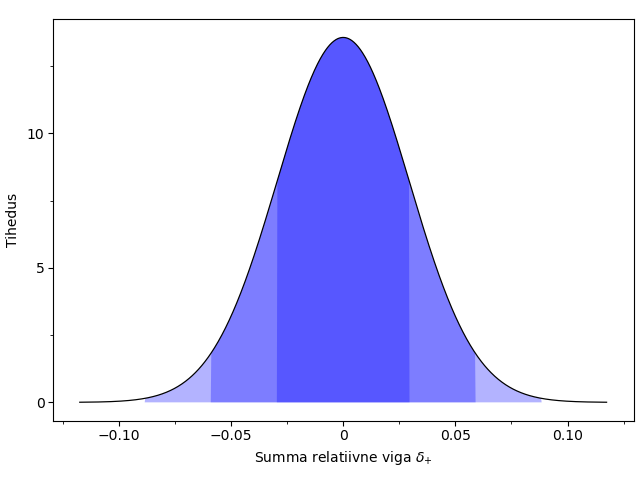
\includegraphics[width=0.8\textwidth]{summa_relatiivne_viga}
    \end{center}
    \caption{Summa relatiivse vea tihedus juhul $x \sim \mathcal{N}(0{,}8; 0{,}04)$, $y \sim \mathcal{N}(0{,}9; 0{,}03)$.}
    \label{fig:summa relatiivne viga tihedus}
\end{figure}

Kuna veakomponentide $\varepsilon_x$ ja $\varepsilon_y$ puhul eeldame normaaljaotust, saame normaaljaotuse omadusi kasutades arvutada, mis tõenäosusega viga $\delta_{+}$ või $\delta_{-}$ mingisse vahemikku jääb. Näiteks täpsete väärtuste $x_0 = 0{,}8$, $y_0 = 0{,}9$ ning absoluutsete vigage $\varepsilon_x \sim \mathcal{N}(0; 0{,}04)$, $\varepsilon_y \sim \mathcal{N}(0; 0{,}03)$ korral jääb $x + y$ relatiivne viga tõenäosusega ligikaudu $68\%$ vahemikku $\pm 0{,}029$. Joonisel~\ref{fig:summa relatiivne viga tihedus} on antud näite korral summa $x + y$ relatiivse vea tihedus. Helesiniselt märgitud alad tähistavad standardhälbe täisarvkordseid vahemikke keskväärtuse ümber.

\subsubsection{Korrutise relatiivse vea omadus}
MMõnikord võib lähendatav suurus olla leitav ligikaudsete arvude korrutisena. Näiteks riskülikukujulise põranda pindala leidmiseks peame korrutama põranda laiuse ja pikkuse, mis mõõtemääramatuse või vigase mõõteriista tõttu ei pruugi olla täpsed.

Olgu $x$ ja $y$ ligikaudsed väärtused arvudest $x_0$ ja $y_0$ absoluutsete vigadega vastavalt $\varepsilon_x$ ning $\varepsilon_y$:
\begin{align*}
    x &= x_0 + \varepsilon_x ,\qquad \varepsilon_x \sim \mathcal{N}(0, \sigma_x) \enspace,\\
    y &= y_0 + \varepsilon_y ,\qquad \varepsilon_y \sim \mathcal{N}(0, \sigma_y) \enspace,
\end{align*}
kus vead $\varepsilon_x$ ja $\varepsilon_y$ on sõltumatud. Suuruste $x$ ja $y$ korrutise relatiivne viga avaldub kujul
\begin{align*}
    \delta &= \frac{x \cdot y - x_0 \cdot y_0}{x_0 \cdot y_0} = \frac{(x_0 + \varepsilon_x) \cdot (y_0 + \varepsilon_y) - x_0 \cdot y_0}{x_0 \cdot y_0} \\
    &= \frac{x_0 \cdot \varepsilon_y + y_0 \cdot \varepsilon_x + \varepsilon_x \cdot \varepsilon_y}{x_0 \cdot y_0} = \frac{\varepsilon_y}{y_0} + \frac{\varepsilon_x}{x_0} + \frac{\varepsilon_x}{x_0} \cdot \frac{\varepsilon_y}{y_0} \enspace.
\end{align*}
Vigade $\varepsilon_x$ ja $\varepsilon_y$ sõltumatuse tõttu on $\delta$ keskväärtus null. Arvestades eelnevat saame tuletada korrutise relatiivse vea dispersiooni
\begin{align*}
    \variance{\delta} &= \mean{\delta^2} - \mean{\delta}^2 = \mean{\delta^2} - 0 \\
    &= \mean{\left( \frac{\varepsilon_y}{y_0} \right)^2 + \left( \frac{\varepsilon_x}{x_0} \right)^2 + \left( \frac{\varepsilon_x}{x_0} \cdot \frac{\varepsilon_y}{y_0} \right)^2 + 2\cdot \frac{\varepsilon_x \cdot \varepsilon_y}{x_0 \cdot y_0} + 2\cdot \frac{\varepsilon_x^2 \cdot \varepsilon_y}{x_0^2 \cdot y_0} + 2\cdot \frac{\varepsilon_x \cdot \varepsilon_y^2}{x_0 \cdot y_0^2}} \\
    &= \mean{\left( \frac{\varepsilon_y}{y_0} \right)^2 + \left( \frac{\varepsilon_x}{x_0} \right)^2 + \left( \frac{\varepsilon_x}{x_0} \cdot \frac{\varepsilon_y}{y_0} \right)^2} \\
    &= \variance{\frac{\varepsilon_y}{y_0}} + \variance{\frac{\varepsilon_x}{x_0}} + \variance{\frac{\varepsilon_y}{y_0}} \cdot \variance{\frac{\varepsilon_x}{x_0}} \enspace.
\end{align*}
Kui $x$ ja $y$ relatiivsete vigade dispersioonid on väikesed on nende korrutis veelgi väiksem. Sellisel juhul saame $\delta$ dispersiooni hinnata küllaltki täpselt, kui jätame korrutise arvutusest välja
\begin{equation}
    \label{eq:korrutise relatiivne viga dispersioon ligikaudne}
    \variance{\delta} \approx \variance{\frac{\varepsilon_y}{y_0}} + \variance{\frac{\varepsilon_x}{x_0}} \enspace.
\end{equation}

\begin{figure}[H]
    \begin{center}
        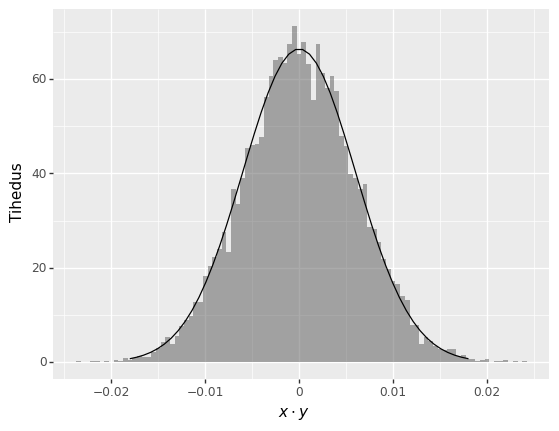
\includegraphics[width=0.8\textwidth]{korrutis_relatiivne_viga}
    \end{center}
    \caption{Korrutise $x\cdot y$ relatiivse vea simuleeritud tihedus histogrammina ja teoreetiline lähendus normaaöjaotsega juhul $x\sim\mathcal{N}(0{,}8; 0{,}004)$, $y \sim \mathcal{N}(0{,}9; 0{,}003)$.}
    \label{fig:korrutis relatiivne viga tihedus}
\end{figure}

Joonisel~\ref{fig:korrutis relatiivne viga tihedus} on histogrammina simuleeritud korrutise $x \cdot y$ relatiivne viga kümnetuhande juhusliku $x$ ja $y$ väärtuse korral, kus $x \sim \mathcal{N}(0{,}8; 0{,}004)$, $y \sim \mathcal{N}(0{,}9; 0{,}003)$. Tume joon on korrutise relatiivse vea lähendus normaaljaotusega tulemuse~\eqref{eq:korrutise relatiivne viga dispersioon ligikaudne} põhjal.

\subsubsection{Jagatise relatiivse vea omadus}
Ligikaudsete väärtuste jagatise puhul on vea edasikandumine keerulisem. Tehese mõned lihtsustavad eeldused saame leida piisavalt täpse hinnangu jagatise relatiivsele veale.

Olgu $x$ ja $y$ ligikaudsed väärtused arvudest $x_0$ ja $y_0$ absoluutsete vigadega vastavalt $\varepsilon_x$ ning $\varepsilon_y$:
\begin{align*}
    x &= x_0 + \varepsilon_x ,\qquad \varepsilon_x \sim \mathcal{N}(0, \sigma_x) \enspace,\\
    y &= y_0 + \varepsilon_y ,\qquad \varepsilon_y \sim \mathcal{N}(0, \sigma_y) \enspace,
\end{align*}
kus vead $\varepsilon_x$ ja $\varepsilon_y$ on sõltumatud. Suuruste $x$ ja $y$ jagatise relatiivne viga avaldub kujul
\begin{equation*}
    \delta = \left( \frac{x}{y} - \frac{x_0}{y_0} \right) \div \frac{x_0}{y_0} = \frac{x \cdot y_0}{y \cdot x_0} - 1 = \frac{y_0}{x_0} \cdot \frac{x_0 + \varepsilon_x}{y_0 + \varepsilon_y} - 1 \enspace.
\end{equation*}
Jagatise relatiivse vea dispersiooni leidmist saame taandada korrutise relatiivse vea dispersioonile, sest $x \div y = x \cdot y^{-1}$. Seega peame hindama $y$ pöördväärtuse relatiivse vea disperisooni
\begin{equation}
    \label{eq:1/y relatiivne viga dispersioon}
    \variance{\left( \frac{1}{y} - \frac{1}{y_0} \right) \div \frac{1}{y_0}} = \variance{\frac{y_0}{y}} = y_0^2 \cdot \variance{\frac{1}{y}} \enspace.
\end{equation}
Taylori arenduse põhjal saame esitada $y^{-1}$ ligikaudselt
\begin{equation*}
    \frac{1}{y} = \frac{1}{y_0 + \varepsilon_y} \approx \frac{1}{y_0} - \frac{1}{y_0^2} \cdot \varepsilon_y \enspace.
\end{equation*}
Tehes eelduse, et $y$ relatiivne viga on väike, on ka Taylori arenduse jääkliige väike.
Vahetulemuse põhjal
\begin{align}
    \variance{\frac{1}{y}}
    &\approx \variance{\frac{1}{y_0} - \frac{1}{y_0^2} \cdot \varepsilon_y} \nonumber \\
    &= \mean{\left( \frac{1}{y_0} - \frac{1}{y_0^2} \cdot \varepsilon_y \right)^2} - \mean{\frac{1}{y_0} - \frac{1}{y_0^2} \cdot \varepsilon_y}^2 \nonumber \\
    &= \frac{1}{y_0^2} + \frac{\sigma_y^2}{y_0^4} - \frac{1}{y_0^2} = \frac{\sigma_y^2}{y_0^4} \enspace. \label{eq:1/y ligikaudne dispersioon}
\end{align}
Tulemuste~\eqref{eq:1/y relatiivne viga dispersioon} ja~\eqref{eq:1/y ligikaudne dispersioon} põhjal saame avaldada $y^{-1}$ relatiivse vea ligikaudse dispersiooni
\begin{equation*}
    \variance{\left( \frac{1}{y} - \frac{1}{y_0} \right) \div \frac{1}{y_0}} \approx y_0^2 \cdot \frac{\sigma_y^2}{y_0^4} = \variance{\frac{\varepsilon_y}{y_0}} \enspace.
\end{equation*}
Seega väikese $y$ relatiivse vea korral on $x$ ja $y$ jagatise relatiivse vea dispersioon, ligikaudu võrdne korrutise omaga
\begin{equation}
    \label{eq:jagatis relatiivne viga dispersioon}
    \variance{\delta} \approx \variance{\frac{\varepsilon_x}{x_0}} + \variance{\frac{\varepsilon_y}{y_0}} + \variance{\frac{\varepsilon_x}{x_0}} \cdot \variance{\frac{\varepsilon_y}{y_0}} \approx \variance{\frac{\varepsilon_x}{x_0}} + \variance{\frac{\varepsilon_y}{y_0}} \enspace.
\end{equation}

\begin{figure}[H]
    \begin{center}
        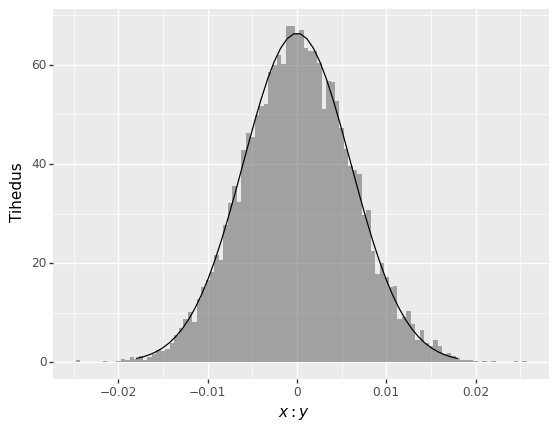
\includegraphics[width=0.8\textwidth]{jagatis_relatiivne_viga}
    \end{center}
    \caption{Jagatise $x:y$ relatiivse vea simuleeritud tihedus histogrammina ja teoreetiline lähendus normaaljaotsega juhul $x \sim \mathcal{N}(0{,}8; 0{,}004)$, $y \sim \mathcal{N}(0{,}9; 0{,}003)$.}
    \label{fig:jagatis relatiivne viga tihedus}
\end{figure}

Joonisel~\ref{fig:jagatis relatiivne viga tihedus} on histogrammina simuleeritud jagatise $x \div y$ relatiivne viga kümnetuhande juhuslikult genereeritud $x$ ja $y$ väärtuse puhul, kus $x \sim \mathcal{N}(0{,}8; 0{,}004)$ ning $y \sim \mathcal{N}(0{,}9; 0{,}003)$. Tume joon on  relatiivse vea lähendus normaaljaotusega tulemuse~\eqref{eq:jagatis relatiivne viga dispersioon} põhjal.
\section{Masinõppe meetodite kvaliteedimõõtude veahinnangud}
\label{section:kvaliteedimõõtude veahinnangud}
Klassifitseerimismeetodite puhul kolm laialdaselt kasutatud kvaliteedimõõtu on õigsus, täpsus ja saagis. Õigsus näitab, kui sagedasti meetod andmepunkte õigesti klassifitseerib (tähistatakse $\accuracy$). Täpsus mõõdab päris positiivsete klassifikatsioonide sagedust ennustatud positiivsete seast (tähistatakse $\precision$). Saagis on päris positiivsete klassifikatsioonide sagedus positiivsete andmepunktide seast (tähistatakse $\recall$).

Tähistagu $i$-ndat andmepunkti elementide paar $(x_i, y_i)$, kus $x_i$ tähistab andmepunkti tunnuseid ning $y_i$ andmepunkti klassi. Antud töös vaatleme ainult binaarse klassifitseerimisülesannet, kus märgend $y_i$ võib olla üks kahest võimalikust väärtusest, negatiivne klass tähistusega $0$ või positiivne klass tähistusega $1$. Tihti vaadatakse meetodi käitumist andmepunktidel. Meetodi $A$ puhul andmepunktile vastav klassifikatsioon on $A(x_i)=a_i$. Juhusliku andmepunkti võib vaadelda juhusliku suurusena $(X, Y)$ ning meetodi klassifikatsiooni selle tunnustel  kui juhuslikku suurust $A$. Seega on võimalik meetodi $A$ kvaliteedimõõdud defineerida läbi ooteväärtuste
\begin{align}
    \accuracy&=\mean{A=Y} \enspace, \label{eq:õigsus}\\
    \precision&=\mean{A=Y|A=1} \enspace, \label{eq:täpsus}\\
    \recall&=\mean{A=Y|Y=1} \enspace. \label{eq:saagis}
\end{align}

Klassifitseerimismeetodi kvaliteedimõõtude tegelikke väärtusi on praktikas peaaegu võimatu leida. Sageli leitakse neile lähendid rakendades meetodit lõplikul hulgal märgendatud testandmetel.

\subsection{Õigsuse lähend}
Õigsuse, täpsuse ja saagise puhul osutub nende kõigi analüüs analoogseks. Samas on õigsuse uurimine tehniliselt kõige lihtsam, sest definitsiooni järgi ei sisalda see tinglikku jaotust. Seetõttu on antud töös õigsust uuritud esimesena.
 
Meetodi rakendamise tulemust valimi $i$-ndal andmepunktil saab tõlgendada kui Bernoulli katset ehk Bernoulli jaotusega juhuslikku suurust $Z_i=[a_i=y_i]$, mille võimlalikud väärtused on $1$ ja $0$ vastavalt õige ning vale klassifikatsiooni korral. Meetodi tegelik õigsus $\accuracy$ määrab juhusliku valimi korral iga katse õnnestumise tulemuse
\begin{equation*}
    \accuracy=\mean{A=Y}=0\cdot\prob{A\neq Y}+1\cdot\prob{A=Y}=\prob{a_i=y_i} \enspace.
\end{equation*}

Lähtudes eelnevast on meetodi õigsus \eqref{eq:õigsus} lähendatav statistilise tõenäosusena üle $N$ andmepunkti suuruse valimi
\begin{equation}
    \label{eq:õigsus lähend}
    \widehat{\accuracy}=\frac{1}{N}\cdot\sum^{N}_{i = 1}Z_i=\frac{1}{N}\cdot\sum^{N}_{i = 1}[a_i=y_i] \enspace.
\end{equation}
Kasutades keskväärtuse, dispersiooni ja Bernoulli jaotuse omadusi saab leida õigsuse lähendi keskväärtuse ning dispersiooni
\begin{align*}
    \mean{\widehat{\accuracy}}&=\frac{1}{N}\cdot\mean{\sum^{N}_{i=1}Z_i}=\frac{1}{N}\cdot N\cdot \accuracy=\accuracy \enspace, \\
    \variance{\widehat{\accuracy}}&=\frac{1}{N^2}\cdot\variance{\sum^{N}_{i=1}Z_i}=\frac{1}{N}\cdot \accuracy\cdot(1-\accuracy) \enspace.
\end{align*}

Kuna suurus $\widehat{\accuracy}$ on ligikaudne väärtus tegelikust õigsusest, on otstarbekas valida piisavalt suur valim, et lähendi absoluutne viga $\Delta\accuracy=\widehat{\accuracy}-\accuracy$ oleks üle valimi küllaltki suure tõenäosusega absoluutväärtuselt võimalikult väike.

\subsection{Täpsuse ja saagise lähendid}
Populatsiooni või valimi korral, mille klasside sagedus ei ole tasakaalus, võib õigsus olla eksitav hinnang meetodi kvaliteedi kohta. Valimis, mille andmepunktidest 90\% kuuluvad positiivsesse ning 10\% negatiivsesse klassi, kõikide andmepunktide positiivseks klassifitseerimine annab õigsuse $\accuracy=0{,}9$. Lisaks hindab õigsus kõiki klassifitseerimisel tehtud vigu ühtemoodi. Kui valepositiivne või valenegatiive klassifikatsioon võib põhjustada tõsiseid tagajärgi on oluline tehtud vigu üksteisest eristada.

Täpsus mõõdab päris positiivsete klassifikatsioonide sagedust ennustatud positiivsete seast. Täpsuse hindamiseks läbi statistilise tõenäosuse on kõigepealt vaja leida kuidas see avaldub tõenäosuste kaudu
\begin{align}
    \precision&=\mean{A=Y|A=1}=0\cdot\prob{A\neq Y|A=1}+1\cdot\prob{A=Y|A=1} \nonumber\\
    &=\prob{Y=1|A=1}=\frac{\prob{Y=1\land A=1}}{\prob{A=1}} \enspace. \label{eq:täpsus tõenäosusesitus}
\end{align}
Tulemuse \eqref{eq:täpsus tõenäosusesitus} põhjal on võimalik leida hinnang täpsusele \eqref{eq:täpsus} üle $N$ andmepunkti suuruse valimi
\begin{equation}
    \label{eq:täpsus lähend}
    \widehat{\precision}=\frac{\frac{1}{N}\cdot\sum\limits_{i=1}^{N}[a_i=1]\cdot[y_i=1]}{\frac{1}{N}\cdot\sum\limits_{i=1}^{N}[a_i=1]}=\frac{\sum\limits_{i=1}^{N}[a_i=1]\cdot[y_i=1]}{\sum\limits_{i=1}^{N}[a_i=1]}\enspace.
\end{equation}

Saagis on päris positiivsete klassifikatsioonide sagedus positiivsete andmepunktide seast. Sarnaselt täpsuse tõenäosusesitusele \eqref{eq:täpsus tõenäosusesitus} saab saagise esitada tõenäosuste kaudu
\begin{equation*}
    \recall=\mean{A=Y|Y=1}=\frac{\prob{Y=1\land A=1}}{\prob{Y=1}} \enspace,
\end{equation*}
mille põhjal on saagise \eqref{eq:saagis} lähend üle valimi arvutatav järgnevalt
\begin{equation}
    \label{eq:saagis lähend}
    \widehat{\recall}=\frac{\frac{1}{N}\cdot\sum\limits_{i=1}^{N}[a_i=1]\cdot[y_i=1]}{\frac{1}{N}\cdot\sum\limits_{i=1}^{N}[y_i=1]}=\frac{\sum\limits_{i=1}^{N}[a_i=1]\cdot[y_i=1]}{\sum\limits_{i=1}^{N}[y_i=1]} \enspace.
\end{equation}

Sellisel kujul esitatud lähendite tõenäosuslik hindamine võib olla keeruline, sest nii murru lugejas kui ka nimetajas on ligikaudsed suurused. Lihtsam on uurida lähendit üle valimi tinglikust jaotusest. Antud juhul on tingimus kvaliteedimõõdu definitsioonis olev sündmus, näiteks täpsuse puhul $A=1$. Tinglikule jaotusele vastava valimi leidmiseks saab kasutada valikumeetodit (\emph{rejection sampling}):
\begin{enumerate}
    \item Võta jaotusest juhuslik andmepunkt.
    \item Kontrolli andmepunkti vastavust tingimusele.
    \item Kui andmepunkt vastab tingimusele võta see valimisse vastasel juhul mitte.
    \item Korda kuni on leitud soovitud koguses tingimusele vastavaid andmepunkte.
\end{enumerate}

Valikumeetodi põhjal on leitav valim $A^{+}$, mis koosneb positiivseks klassifitseeritud andmepunktidest, ning valim $Y^{+}$, mis koosneb positiivse klassiga andmepunktidest. Kasutades vastavaid valimeid on lähendid \eqref{eq:täpsus lähend} ja \eqref{eq:saagis lähend} esitatavad kujul:
\begin{align}
    \widehat{\precision}&=\frac{1}{|A^{+}|}\cdot\sum_{i\in A^{+}}[y_i=1] \enspace, \label{eq:täpsus tinglik lähend}\\
    \widehat{\recall}&=\frac{1}{|Y^{+}|}\cdot\sum_{i\in Y^{+}}[a_i=1] \label{eq:saagis tinglik lähend}\enspace.
\end{align}
On oluline tähele panna, et lähendid \eqref{eq:täpsus tinglik lähend} ja \eqref{eq:saagis tinglik lähend} on analoogsed õigsuse lähendile \eqref{eq:õigsus lähend} ning on seetõttu on nende absoluutsed ja relatiivsed vead samasuguste omadustega.

Lihtsa valikumeetodi puhul võib osutuda probleemseks tingimuse kontrollimine valimi moodustamisel. Täpsuse puhul on tingimuse kontrollimine lihtne, sest piisab vaid meetodi rakendamisest andmepunktile. Saagise puhul ei pruugi meetod väga hästi toimida, sest tingimuse kontrollimiseks peab välja selgitama andmepunkti tegeliku klassi. Tegeliku klassi leidmine on võrreldes klassifikatsiooni leidmisega kulukas. Valikumeetodi rakendamine saagise lähendamiseks on eriti kulukas, kui positiivse klassiga andmepunktid jaotuses on haruldased. Leidub ülesandeid mille puhul võib positiivse juhtumi esinemissagedus olla $1:10 000$ nagu tekstist faktide eraldamine. Sellisel juhul on $1 000$ elemendilise valimi leidiseks vaja märgendada $10$ miljonit andmepunkti. Isesõitvate autode puhul võivad huvipakkuvad sündmused esineda ühel korral miljonist ning seega on naiivse lähenemise korral vaja märgendada ligi miljard andmepunkti. Kuid vajaliku töökindluse saavutamiseks peab selliseid sündmusi ikkagi arvestama. See on ka üks põhjus, miks suure töökindlusega praktikas kasutatavate masinõppe algoritmide loomine on keerukas protsess.

\subsection{Õigsuse lähendi absoluutne viga}
Valimi põhjal leitud lähendid kvaliteedimõõtudele sisaldavad viga. Veendumaks lähendi vastavuses selle täpsele väärtusele tekib küsimus vea suuruse kohta. Vea arvutamiseks peab teadma täpset väärtust, mis ei pruugi olla võimalik. Täpset väärtust teadmata saab viga hinnata tõenäosuslikult. Sageli seatakse eesmärgiks hinnata kui suur on viga $95\%$ juhtudest.

Üks viis vea tõenäosuslikuks hindamiseks on kasutada konsentratsioonivõrratusi, näiteks Höffdingi võrratust. Höffdingi võrratus on suurte arvude seaduse konkreetne erijuht, mis annab üldistest hinnangutest täpsemaid tõkkeid tõenäosustele. Höffdingi võrratus sätib ülemise tõkke tõenäosusele, et tõkestatud paarikaupa sõltumatute juhuslike suuruste summa erineb selle summa keskväärtusest (oodatud väärtusest) vähemalt mingi konstandi võrra \cite{höffdingi-võrratus,tõenäosusteooria-2-loengukonspekt}. Täpsemalt, kui juhuslikud suurused $Z_1,Z_2,\dots,Z_N$ on sõltumatud ning leiduvad tõkked
\begin{equation*}
    a_i\leq Z_i\leq b_i \enspace, 
\end{equation*}
siis summa $S_N=Z_1+\cdots+Z_N$ ning iga positiivse $c$ korral
\begin{equation*}
    \prob{| S_N - \mean{S_N} | \geq c} \leq 2 \exp{\left( - \frac{2 c^2}{\sum_{i = 1}^{N}(b_i - a_i)^2}\right)} \enspace .
\end{equation*}

Kuna Bernoulli jaotusega juhuslike suuruste jaoks leiduvad tõkked $0\leq Z_i\leq1$ järeldub Höffdingi võrratusest seos
\begin{equation}
    \label{eq:höffding absoluutne viga}
    \prob{\mid \widehat{\accuracy} - \accuracy \mid \geq \frac{c}{N}} \leq 2 \exp{\left( - \frac{2 c^2}{N} \right)} \enspace,
\end{equation}
mille põhjal saab hinnata lähendi $\widehat{\accuracy}$ absoluutse vea alumise tõkke tõenäosust. Sättides võrratuse \eqref{eq:höffding absoluutne viga} parema poole võrdseks olulisusega $\alpha$ avaldub veahinnangu alumine tõke kujul
\begin{equation*}
     \varepsilon := \frac{c}{N} = \sqrt{- \frac{1}{2 N} \cdot \ln{\left( \frac{\alpha}{2} \right)}} \enspace.
\end{equation*}
Tulemust kasutades on võimalik leida valimi vajalik suurus
\begin{equation*}
    N \geq -\frac{1}{2\varepsilon^2}\cdot\ln{\left(\frac{\alpha}{2}\right)} \enspace,
\end{equation*}
et fikseeritud olulisuse korral saavutada soovitud suurusega veahinnang.

\begin{table}[H]
    \centering
    \caption{Valimi suurused kindluse ning absoluutse vea suhtes Höffdinig võrratuse põhjal. Kindluse puhul on sulgudes tähistatud, mitu normaaljaotuse standardhälvet keskväärtuse ümbruses see katab.}
    \begin{tabular}{l | r r r}
        $1-\alpha$ & $\varepsilon=10\%$ & $\varepsilon=1\%$ & $\varepsilon=0{,}1\%$ \\
    	\hline
    	$99\% \enspace (3\sigma)$ & $265$ & $26492$ & $2649159$ \\
    	$95\% \enspace (2\sigma)$ & $185$ & $18445$ & $1844440$ \\
    	$68\% \enspace (1\sigma)$ & $92$  & $9163$  & $916291$  \\
    \end{tabular}
    \label{tab:höffding absoluutne viga}
\end{table}

\begin{figure}[H]
    \begin{center}
        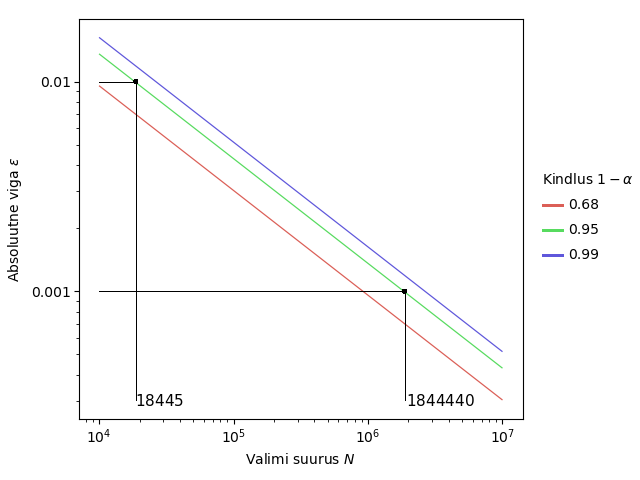
\includegraphics[width=\textwidth]{hoeffding_absoluutne_viga.png}
    \end{center}
    \caption{Valimi suurused olulisuse ning absoluutse vea suhtes Höffdinig võrratuse põhjal kindlusega $1-\alpha$.}
    \label{fig:höffding absoluutne viga}
\end{figure}

Tabelis \ref{tab:höffding absoluutne viga} on välja toodud vajalik valimi suurus soovitud kindluse ja lähendi absoluutse vea suhtes Höffdingi võrratuse põhjal, kindluse puhul on sulgudes tähistatud, kui mitu normaaljaotuse standardhälvet $\sigma$ keskväärtuse ümbruses see katab. Näiteks kui on soov olla $95\%$ kindel, et valimi põhjal arvutatud õigsus $\widehat{\accuracy}$ erineb algoritmi tegelikust õigsusest kuni ühe protsendi võrra, peab õigsust hindama valimil suurusega vähemalt $18504$. Joonisel \ref{fig:höffding absoluutne viga} on sama mõttekäik esitatud graafiliselt.

Õigsuse lähendi absoluutse vea hindamiseks saab ka kasutada asjaolu, et suurused $Z_i$ on Bernoulli jaotusega. See tähendab, et summa
\begin{equation*}
    S_N=\sum^{N}_{i = 1}Z_i \enspace,
\end{equation*}
on binoomjaotusega. Mingi binoomjaotusega juhusliku suuruse $X$ puhul tähistatakse seda $X\sim\mathcal{B}(n, p)$, kus parameeter $n$ on Bernoulli katsete arv ja $p$ katse õnnestumise tõenäosus. Sellest lähtudes saab väita järgnevat
\begin{equation*}
    S_N\sim\mathcal{B}(N, \accuracy) \enspace.
\end{equation*}
Seega on õigsuse lähend $\widehat{\accuracy}$ skaleeritud binoomjaotusega juhuslik suurus. Eespool uuritud Höffdingi võrratusel põhinevad tõkked selle omadusega ei arvestanud ning olid binoomjaotuse parameetrist $p$ sõltumatud, tegu oli konservatiivse hinnanguga. Höffidngi võrratus on universaalne üle kõikide binoomjaotuse parameetrite $p$, millest halvim variant realiseerub juhul $p=0{,}5$. Binoomjaotusel põhinevad tõkked on täpsed ning annavad aimu Höffidngi võrratuse tulemuste ebatäpsustest. Lisaks näitavad binoomjaotusel põhinevad arvutused kuidas meetodi tegelik õigsus $\accuracy$ mõjutab tulemusi.

Kasutades teadmist, et uuritav summa on binoomjaotusega saab leida jaotuse parameetritest sõltuva hinnangu. Olulisuse $\alpha$ korral saab absoluutse veahinnangu tõkke $\varepsilon$ arvutada lähtudes võrrandist
\begin{equation}
    \label{eq:binoomjaotus absoluutne viga}
    \prob{\mid\widehat{\accuracy}-\accuracy\mid\geq\varepsilon}=\alpha \enspace,
\end{equation}
ning valides protsendipunktid sümmeetriliselt
\begin{align*}
    \prob{\widehat{\accuracy} \leq \accuracy-\varepsilon} &= \frac{\alpha}{2} \enspace,\\
    \prob{\widehat{\accuracy} <    \accuracy+\varepsilon} &= 1 - \frac{\alpha}{2} \enspace,
\end{align*}
millest binoomjaotusega juhusliku suuruse $S_N$ eraldamisel ühele poole võrratuse märki saab
\begin{align*}
    \prob{S_N \leq N \cdot(\accuracy-\varepsilon)} &= \frac{\alpha}{2} \enspace,\\
    \prob{S_N < N \cdot(\accuracy+\varepsilon)} &= 1 - \frac{\alpha}{2} \enspace.
\end{align*}
Paremale poole võrratuse märki tekkinud avaldised on $S_N$ jaotuse vastavalt $\frac{\alpha}{2}$ ja $1-\frac{\alpha}{2}$ protsendipunktid, ehk väärtused, millest $S_N$ võtab väiksemaid väärtusi protsendipunktile vastava tõenäosusega
\begin{align*}
    q_1 &= N \cdot(\accuracy-\varepsilon) \enspace, \\
    q_2 &= N \cdot(\accuracy+\varepsilon) \enspace. \\
\end{align*}
Fikseeritud olulisuse ja binoomjaotuse parameetrite korral on protsendipunkt arvutatav kasutades $S_N$ jaotuse omadusi. 

Absoluutse vea tõkkeks $\varepsilon$ võrrandist \eqref{eq:binoomjaotus absoluutne viga} on valitud suurem protsentipunktide põhjal arvutatud veahinnang
\begin{equation}
    \label{eq:binoomjaotus absoluutne viga tõke}
    \varepsilon = \max \left( \accuracy - \frac{q_1}{N} , \frac{q_2}{N} - \accuracy \right) \enspace.
\end{equation}
Parameetri $N$ kasvades koondub binoomjaotus normaaljaotuseks \cite{tõenäosusteooria-algkursus}. Seega suuremate $N$ väärtuste puhul muutub binoomjaotus sümmeetriliseks, järelikult erinevad $q_1$ ja $q_2$ põhjal arvutatud veahinnangute väärtused tegelikkuses vähe. Tulemust \eqref{eq:binoomjaotus absoluutne viga tõke} kasutades saab arvutada vajaliku valim suuruse soovitud olulisuse suhtes, kuid selle jaoks peab tegema mudeli tegeliku õigsuse $\accuracy$ kohta oletusi.

\begin{table}[H]
    \centering
    \caption{Valimi suurused absoluutse vea ning oletatava õigsuse suhtes binoomjaotuse põhjal kindlusega $95\%$. Sulgudes on näidatud kui mitu korda Höffdingi võrratusel põhinev valim suurem on.}
    \begin{tabular}{l | r r r}
        $\accuracy$ & $\varepsilon = 10\%$ & $\varepsilon = 1\%$ & $\varepsilon = 0,1\%$ \\
    	\hline
    	$70\%$ & $75\enspace(2{,}47)$ & $8100\enspace(2{,}28)$ & $806289\enspace(2{,}29)$ \\
    	$90\%$ & $35\enspace(5{,}29)$ & $3600\enspace(5{,}12)$ & $347020\enspace(5{,}32)$ \\
    	$95\%$ & $20\enspace(9)$      & $1850\enspace(9{,}97)$ & $183285\enspace(10{,}06)$ \\
    \end{tabular}
    \label{tab:binoomjaotus absoluutne viga}
\end{table}

\begin{figure}[H]
    \begin{center}
        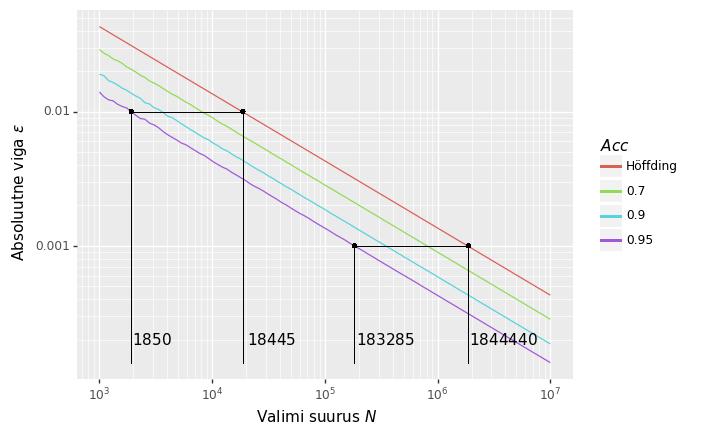
\includegraphics[width=\textwidth]{binoomjaotus_absoluutne_viga.png}
    \end{center}
    \caption{Valimi suurused absoluutse vea ning oletatava õigsuse suhtes binoomjaotuse põhjal kindlusega $95\%$.}
    \label{fig:binoomjaotus absoluutne viga}
\end{figure}

Tabelis \ref{tab:binoomjaotus absoluutne viga} ja joonisel \ref{fig:binoomjaotus absoluutne viga} on esitatud valimi vajalikud suurused meetodi oletatud õigsuse ja absoluutse veahinnangu soovitud suuruse suhtes binoomjaotuse omaduste põhjal kindlusega $95\%$. Võrdluseks on välja toodud ka Höffdingi võrratusel põhinevad tulemused sama kindlusega, joonisel on see esitatud eraldi joonega, tabelis on sulgudes kirjas kui mitu korda on Höffdingi võrratuse põhine valim suurem. Eeldusel, et algoritmi tegelik õigsus on $90\%$, absoluutse vea kuni üks protsent jaoks läheb vaja valimit suurusega $3600$, mis on umbes viis korda väiksem kui valim, mida on vaja Höffdingi võrratuse põhjal.

\subsection{Õigsuse lähendi relatiivne viga}
Lisaks ligikaudse väärtuse absoluutsele veale kasutatakse lähendi headuse mõõtmiseks relatiivset viga. Õigsuse lähendi relatiivse vea keskväärtus ja dispersioon avalduvad järgnevalt
\begin{align*}
    \mean{\frac{\widehat{\accuracy}}{\accuracy}-1}&=\frac{1}{\accuracy}\cdot\mean{\widehat{\accuracy}}-1=1-1=0 \nonumber\enspace, \\
    \variance{\frac{\widehat{\accuracy}}{\accuracy}-1}&=\frac{1}{\accuracy^2}\cdot\frac{\accuracy\cdot(1-\accuracy)}{N}=\frac{1}{N}\cdot\frac{1-\accuracy}{\accuracy} \enspace.
\end{align*}
Uurides lähendi relatiivse ja absoluutse vea hajuvuse suhet
\begin{equation*}
    \variance{\frac{\widehat{\accuracy}}{\accuracy}} : \variance{\widehat{\accuracy}-\accuracy}=
    \left( \frac{1}{N}\cdot\frac{1-\accuracy}{\accuracy} \right) : \left( \frac{1}{N}\cdot \accuracy\cdot(1-\accuracy) \right)=\frac{1}{\accuracy^2} \enspace,
\end{equation*}
selgub, et kõrge õigsuse korral on õigsuse lähendi vead ligikaudu sama hajuvusega.

Nagu absoluutse veahinnangu puhul on ka relatiivse veahinnangu puhul eesmärk seda absoluutväärtuselt minimeerida. Seega võib küsida kui suurt valimit läheb vaja, et piisavalt suure kindlusega oleks relatiivne viga võimalikult väike.

Õigsuse lähend sisaldab binoomjaotusega juhuslikku suurust. Järelikult on võimalik relatiivset viga tõenäosuslikult hinnata kasutades binoomjaotuse omadusi. Lähtudes võrrandist
\begin{equation}
    \label{eq:binoomjaotus relatiivne viga}
    \prob{\left|\frac{\widehat{\accuracy}}{\accuracy}-1\right|\geq\varepsilon}=\alpha \enspace,
\end{equation}
millest tõenäosusmärgi aluses võrratuses eraldada binoomjaotusega juhusliku suuruse $S_N$ ühele poole võrratusemärki
\begin{align*}
    \prob{S_N \leq N \cdot \accuracy \cdot (1-\varepsilon)} &= \frac{\alpha}{2} \enspace, \\
    \prob{S_N <    N \cdot \accuracy \cdot (1+\varepsilon)} &= 1 - \frac{\alpha}{2} \enspace,
\end{align*}
avalduvad olulisusele vastavad protsendipunktid kujul
\begin{align*}
    q_1 &= N \cdot \accuracy \cdot (1-\varepsilon) \enspace, \\
    q_2 &= N \cdot \accuracy \cdot (1+\varepsilon) \enspace.
\end{align*}

Relatiivse vea tõkkeks $\varepsilon$ võrrandist \eqref{eq:binoomjaotus relatiivne viga} on valitud suurem protsendipunktide põhjal avalduv veahinnang
\begin{equation*}
    \varepsilon = \max \left( 1 - \frac{q_1}{N\cdot\accuracy} , \frac{q_2}{N\cdot\accuracy} - 1 \right) \enspace.
\end{equation*}
Tulemuse põhjal saab arvutada valimi vajalikud suurused olulisuse suhtes.

\begin{table}[H]
    \centering
    \caption{Valimi suurused relatiivse vea ning eeldatud õigsuse suhtes binoomjaotuse põhjal kindlusega $95\%$.}
    \begin{tabular}{l | r r r }
        $\accuracy$ & $\varepsilon=10\%$ & $\varepsilon=1\%$ & $\varepsilon=0{,}1\%$ \\
    	\hline
    	$70\%$ & $161$ & $16331$ & $1646727$ \\
    	$90\%$ & $53$  & $4176$  & $425856$  \\
    	$95\%$ & $20$   & $1926$  & $202223$  \\
    \end{tabular}
    \label{tab:binoomjaotus relatiivne viga}
\end{table}

\begin{figure}[H]
    \begin{center}
        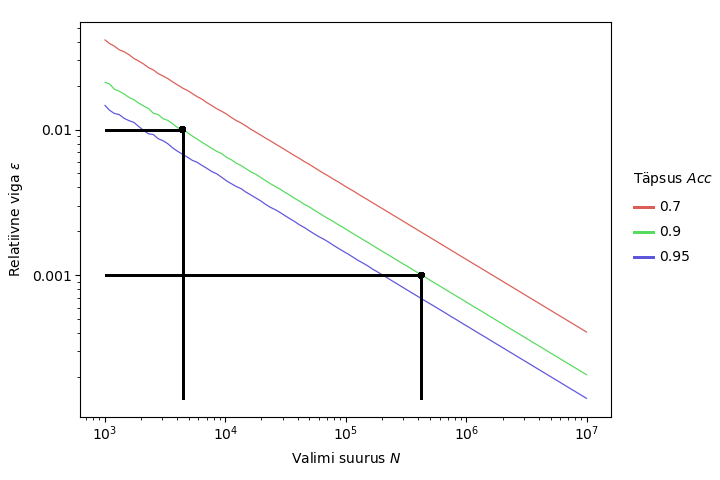
\includegraphics[width=\textwidth]{binoomjaotus_relatiivne_viga.png}
    \end{center}
    \caption{Valimi suurused relatiivse vea ning eeldatud õigsuse suhtes binoomjaotuse põhjal kindlusega $95\%$.}
    \label{fig:binoomjaotus relatiivne viga}
\end{figure}

Tabelis \ref{tab:binoomjaotus relatiivne viga} ja joonisel \ref{fig:binoomjaotus relatiivne viga} on esitatud valimi vajalikud suurused meetodi oletatud õigsuse ja relatiivse veahinnangu soovitud suuruse suhtes binoomjaotuse omaduste põhjal kindlusega $95\%$.

\subsection{Tulemuste empiiriline testimine}
Teoreetilisi tulemusi on alati hea praktikas kontrollida. Niimoodi on võimalik leide lihtsasti valideerida ning ka avastada enamuse arvutusvigadest.

\begin{figure}[H]
    \begin{center}
        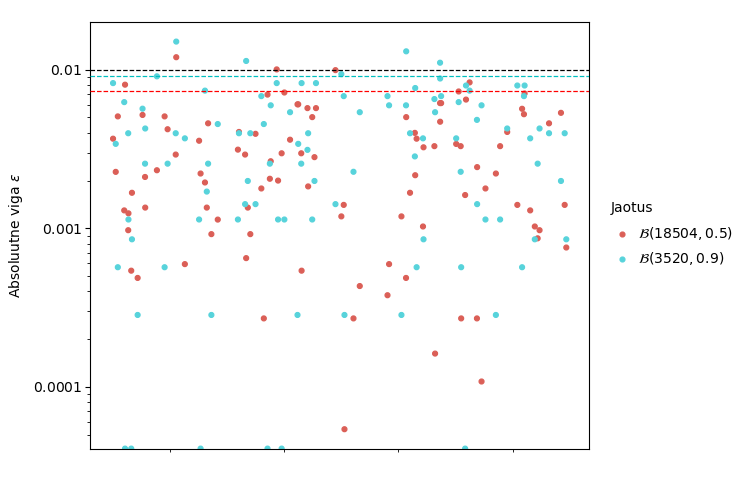
\includegraphics[width=\textwidth]{absoluutne_viga_statistiline_test.png} 
    \end{center}
    \caption{Höffdingi võrratusel (punane) ja binoomjaotusel (sinine) põhinevate veahinnangute empiiriline test lähendi veaga kuni $1\%$ saamiseks kindlusega $95\%$. Binoomjaotusega summad $S_N$ õigsuse hinnangutes on juhuslikult genereeritud vastavatest jaotustest, punktid joonisel tähistavad summale vastava õigsuse hinnangu absoluutse vea absoluutväärtust. Värvilised jooned tähistavad empiiriliselt saadud $0{,}95$ protsendipunkte, must joon nende oodatud asukohta.}
    \label{fig:höffding ja binoomjaotus absoluutne viga empiiriline test}
\end{figure}

Näiteks Höffdingi võrratuse põhjal kindlusega $95\%$ kuni ühe protsendise absoluutse veahinnanguga õigsuse lähendi saavutamiseks on vaja valimit suurusega $18504$. Eeldusel, et klassifitseerimismeetodi tegelik õigsus on $90\%$ on binoomjaotuse hinnangu põhjal vaja selleks $3520$ andmepunkti. Joonisel \ref{fig:höffding ja binoomjaotus absoluutne viga empiiriline test} on kujutatud antud näite empiiriline test, kus summa
\begin{equation*}
    S_N=\sum_{i=1}^N Z_i \enspace,
\end{equation*}
on juhuslikult genereeritud jaotusest $\mathcal{B}(18504; 0{,}5)$ Höffdingi võrratuse puhul (punane) ning $\mathcal{B}(3520; 0{,}9)$ binoomjaotuse hinnangu puhul (sinine). Punktid joonisel tähistavad summal põhineva lähendi absoluutset viga
\begin{equation*}
    \varepsilon=\left|\frac{S_N}{N}-p\right|=\left|\widehat{\accuracy}-\accuracy\right| \enspace,
\end{equation*}
must joon veahinnangu absoluutväärtuse ülemist tõket, millest saadud veahinnang $\varepsilon$ peaks olema väiksem $95\%$ juhtudest. Punane ja sinine joon on vastava jaotuse puhul tõmmatud läbi empiirilise testimise tulemusel saadud punkti, millest $95\%$ jäävad allapoole. Binoomjaotuse hinnang on täpne ning langes ka antud juhul oodatule lähedale. See-eest langes punane joon oodatust allapoole. Kuna Höffdingi võrratus ülehindab valimi valjalikku suurust on punase joone langemine tema oodatud asukohast allapoole loomulik, sest suurem valim tähendab täpsemat lähendit ja seega väiksemat viga.

\section{Masinõppe meetodite kvaliteedimõõtude võrdlus}
Uue meetodi kasutusele võtmine tähendab, et on olemas vanem juba kasutuses meetod. Võib osutuda otstarbekaks kasutada vanemat meetodit uue hindamisel. Vana meetodi asendamisel on eelkõige tähtis kas ja kui palju on uus meetod eelmisest parem. Väljaselgitamiseks võib uurida meetodite kvaliteedimõõtude vahesid.

Järgnevas laiendame eelmises peatükis sisse toodud tähistusi. Tähistagu $i$-ndat andmepunkti elementide paar $(x_i, y_i)$, kus $x_i$ tähistab andmepunkti tunnuseid ning $y_i$ andmepunkti klassi. Olgu $A$ uus ning $B$ varasem klassifitseerimismeetod, siis saame tähistada andmepunktile vastavad klassifikatsioone  $A(x_i)=a_i$ ja $B(x_i)=b_i$. Vaadeldes andmepunkti juhusliku suurusena $(X, Y)$ võib ka meetodite klassifikatsioone sellel vaadelda juhuslike suurustena $A$ ja $B$ ning meetodite kvaliteedimõõdud on defineeritud keskväärtuste kaudu läbi valemite \eqref{eq:õigsus}, \eqref{eq:täpsus} ja \eqref{eq:saagis}. Näiteks meetodi $B$ õigsus on $\accuracy_B=\mean{B=Y}$. Siit lähtuvalt saab meetodite erinevuse uurimisel vaadata meetodite kvaliteedimõõtude vahesid
\begin{align}
    \Delta\accuracy&=\mean{A=Y}-\mean{B=Y} \enspace, \label{eq:õigsus vahe} \\
    \Delta\precision&=\mean{A=Y|A=1}-\mean{B=Y|B=1} \enspace, \label{eq:täpsus vahe} \\
    \Delta\recall&=\mean{A=Y|Y=1}-\mean{B=Y|Y=1} \enspace. \label{eq:saagis vahe}
\end{align}

\subsection{Kvaliteedimõõtude vahede lähendid}
Kuna defineeritud vahede täpseid väärtusi on praktikas keeruline leida hinnatakse neid kasutades valimi keskmisi. Sealjuures on loomulik mõlema meetodi hindamiseks kasutada sama valimit. Ühelt poolt on see standardpraktika - tüüpiliselt hinnatakse masinõppemeetodite edukust fikseeritud testvalimite (\emph{benchmark}) peal. Teisalt tooks kahe valimi kasutamine vajaduse käsitsi märgendada rohkem andmepunkte ning lisab ka lõpptulemusse rohkem juhuslikkust. Kui vastav testvalim sisaldab $N$ andmepunkti, siis saab õigsuste vahe lähendi avaldada järgnevalt
\begin{align}
    \Delta\widehat{\accuracy}&=\frac{1}{N}\cdot\sum_{i=1}^{N}[a_i=y_i]-\frac{1}{N}\cdot\sum_{i=1}^{N}[b_i=y_i] \nonumber\\
    &=\frac{1}{N}\cdot\sum_{i=1}^{N}[a_i=y_i]-[b_i=y_i]\nonumber\\
    &=\frac{1}{N}\cdot\sum_{a_i\neq b_i}[a_i=y_i]-[b_i=y_i] \enspace. \label{eq:õigsus vahe lähend}
\end{align}
Saadud võrduses \eqref{eq:õigsus vahe lähend} on summa märgi all nullist erinev arv parajasti siis, kui meetodite klassifikatsioonid on erinevad. Sellest järeldub, et meetodite õigsuste vahe hindamiseks peab märgendama vaid andmepunkte, kus $a_i\neq b_i$. Näiteks kui meetodid on üle $90\%$ õigsustega võivad nende klassifikatsioonid erineda maksimaalselt $20\%$ andmetest. Sellisel juhul peab märgendama vaid iga viienda andmepunkti. Veelgi enam, kuna iga summa liige valemis  \eqref{eq:õigsus vahe lähend} on $\pm 1$, saab hinnata $\Delta\widehat{\accuracy}$ ilma ühtegi andmepunkti märgendamata
\begin{equation}
    \label{eq:õigsus vahe lähend tõke}
    |\Delta\widehat{\accuracy}|\leq\frac{\#\{i: a_i\neq b_i\}}{N} \enspace,
\end{equation}
kus murru lugejas tähistab $\#$ hulga suurust. Seega on võimalik veenduda, kas kaks algoritmi üldse õigsuse poolest erinevad andmepunktide tegelikke klasse teadmata.

Analoogselt õigsusele võib avaldada ka valimipõhiste täpsushinnangute vahe
\begin{equation}
    \label{eq:täpsus vahe lähend kole}
    \Delta\widehat{\precision}=\frac{\sum\limits_{i=1}^{N}[a_i=1]\cdot[y_i=1]}{\sum\limits_{i=1}^N[a_i=1]}-
    \frac{\sum\limits_{i=1}^{N}[b_i=1]\cdot[y_i=1]}{\sum\limits_{i=1}^N [b_i=1]} \enspace,
\end{equation}
mille edasise lihtsustamise muudab raskeks erinevus murru nimetajates. Kuna tehniliselt ei pea täpsuse hindamisel kasutama sama testvalimit mõlema algoritmi jaoks, siis võib esialgset testvalmit kitsendada nii, et murru lugejad langevad kokku
\begin{equation*}
    \sum\limits_{i=1}^{N_A}[a_i=1]=S=\sum\limits_{i=1}^{N_B}[b_i=1] \enspace,
\end{equation*}
ning $N=\max(N_A, N_B)$.
Selline lähenemine on samaväärne valikumeetodi põhjal kahe $S$ andmepunktise valimi moodustamisega, kus vastuvõtutingimused on vastavalt $a_i=1$ ja $b_i=1$. Seda arvestades saab valemi \eqref{eq:täpsus vahe lähend kole} viia lihtsustatud kujule
\begin{equation}
     \Delta\widehat{\precision}=\frac{1}{S}\cdot\sum\limits_{i=1}^{N_A}[a_i=1]\cdot[y_i=1]-\frac{1}{S}\cdot\sum\limits_{i=1}^{N_B}[b_i=1]\cdot[y_i=1] \enspace,
\end{equation}
kus $a_i$ on määratud vaid esimesel $N_A$ ja $b_i$ on määratud vaid esimesel $N_B$ andmepunktil. Seega on $a_i$ ja $b_i$ väärtus kõigi $N$ punkti seas kas määramata, $0$ või $1$. Siit lähtuvalt
\begin{align}
    \Delta\widehat{\precision}&=\frac{1}{S}\cdot\left(\sum_{\substack{a_i=1\\ b_i=1}}[y_i=1]+\sum_{\substack{a_i=1\\ b_i\neq 1}}[y_i=1]-\sum_{\substack{a_i=1\\ b_i=1}}[y_i=1]-\sum_{\substack{a_i\neq 1\\ b_i=1}}[y_i=1]\right) \nonumber\\
    &=\frac{1}{S}\cdot\left(\sum_{\substack{a_i=1\\ b_i\neq 1}}[y_i=1]-\sum_{\substack{a_i\neq 1\\ b_i=1}}[y_i=1]\right) \nonumber\\
    &=\frac{1}{S}\cdot\sum_{a_i\neq b_i}[a_i=1]\cdot[y_i=1]-[b_i=1]\cdot[y_i=1] \enspace. \label{eq:täpsus vahe lähend}
\end{align}
Andmepunktide märgendamise mõttes on täpsuse vahe lähend \eqref{eq:täpsus vahe lähend} samaväärne õigsuse valemiga \eqref{eq:õigsus vahe lähend}, sest hinnangu arvutamiseks peab märgendama vaid andmepunkte, mille puhul $a_i\neq b_i$.

Täpsuse vahehinnangu praktiline arvutamine algab $S$ fikseerimisest. Seejärel tuleb valimile rakendada meetodeid kuni kumbki on $S$ andmepunkti positiivseks klassifitseerinud. Märgendama peab valimi andmepunktid, mille puhul on olemas mõlema meetodi klassifikatsioonid, mis on üksteisest erinevad. Nüüd on võimalik arvuta summa liikmete väärtused ning seejärel hinnang täpsuste vahele. Sellega on oluliselt vähendatud märgendamist vajavate andmete hulka.

Saagise vahe avaldub sarnaselt täpsusele, lähtudes valemist
\begin{equation*}
    \Delta\widehat{\recall}=\frac{\sum\limits_{i=1}^{N}[a_i=1]\cdot[y_i=1]}{\sum\limits_{i=1}^{N}[y_i=1]}-\frac{\sum\limits_{i=1}^{N}[b_i=1]\cdot[y_i=1]}{\sum\limits_{i=1}^{N}[y_i=1]} \enspace,
\end{equation*}
kus erinevalt täpsusest on murdude nimetajad definitsiooni järgi võrdsed. Tähistagu nimetajas olevat summat
\begin{equation*}
    T=\sum_{i=1}^N[y_i=1] \enspace.
\end{equation*}
Korrates täpsuse valemi \eqref{eq:täpsus vahe lähend} tuletamisega analoogset mõttekäiku, võib esitada saagise vahe hinnangu kujul
\begin{equation}
    \label{eq:saagis vahe lähend}
     \Delta\widehat{\recall}=\frac{1}{T}\cdot\sum_{a_i\neq b_i}[a_i=1]\cdot[y_i=1]-[b_i=1]\cdot[y_i=1] \enspace. 
\end{equation}
Märgendamise seisukohalt on $T$ arvutamine kulukas, kuna iga summa liikme puhul peab teadma andmepunkti tegelikku klassi. Kõigi $N$ andmepunkti manuaalne märgendamine on väga ressursimahukas. 
Alternatiiviks on väiksema valimi põhjal positiivse klassi esinemise sageduse ennustamine. See on võimalik vaid siis kui positiivse klassi esinemise sagedus on piisavalt suur. Kui positiivse klassi esindajad on sagedusega $1:1000$, siis on tarvis adekvaatse hinnangu saamiseks läbi vaadata üle kümnetuhande andmepunkti. Seega on valemi \eqref{eq:saagis vahe lähend} praktiline rakendamine raskendatud veelgi madalama esinemissagedusega sündmuste korral.

\subsection{Õigsuste vahe lähendamine}
Siiani on lähendid kvaliteedimõõtude vahele avaldatud vahetult läbi vahe oodatud väärtuse definitsiooni. Tehes teisendusi vahe definitsioonis antud avaldises on võimalik see eraldada mitmeks komponendiks. Vahe lähendi saamiseks on ka võimalik lähendada iga komponenti eraldi ning nende põhjal arvutada hinnang vahele.

Olgu olemas kaks klassifitseerimismeetodit koos juhusliku andmepunkti $Y$ klassifitseerimisele vastavate juhuslike suurustega $A$ ja $B$. Siis saab valemi \eqref{eq:õigsus vahe} kirjutada lahti vastavalt definitsioonile
\begin{equation}
    \label{eq:õigus vahe definitsiooni järgi keskväärtuste kaudu}
    \Delta\accuracy=\mean{A=Y}-\mean{B=Y}=\mean{[A=Y]-[B=Y]} \enspace.
\end{equation}
Tähistagu $Z$ valemis \eqref{eq:õigus vahe definitsiooni järgi keskväärtuste kaudu} viimase keskväärtusmärgi all olevat juhuslikkus suurust, ehk $Z=[A=Y]-[B=Y]$. Analoogselt võib valemis \eqref{eq:õigsus vahe lähend} oleva summa liikmeid tõlgendada juhuslike suurustena $Z_i=[a_i=y_i]-[b_i=y_i]$. Arvestades, et $Z_i$ on sõltumatud ning sama jaotusega kui $Z$, on lihtne näha, et lähendi \eqref{eq:õigsus vahe lähend} keskväärtus on
\begin{equation}
    \mean{\Delta\widehat{\accuracy}}=\frac{1}{N}\cdot\sum_{i=1}^N\cdot\mean{Z_i}=\Delta\accuracy \enspace.
\end{equation}
See tähendab, et $\widehat{\accuracy}$ on nihketa hinnang õigsuste vahele. Kuna meetodite erinevus avaldub sündmustes, kus meetodite klassifikatsioonid erinevad ($Z\neq 0$), võib $\Delta\accuracy$ avaldada selliste sündmuste kaudu
\begin{align*}
    \Delta\accuracy&=\prob{Z=0}\cdot\mean{Z \mid Z = 0}+\prob{Z \neq 0}\cdot\mean{Z \mid Z \neq 0} \\
    &=\prob{Z \neq 0}\cdot\mean{Z \mid Z \neq 0} \enspace.
\end{align*}
Edasiste arvutuste selgemaks esitamiseks on otstarbekas kasutusele võtta tähistused
\begin{align}
    \beta&=\prob{Z\neq0} \enspace, \label{eq:beta} \\
    \gamma&=\mean{Z \mid Z \neq 0} \enspace, \label{eq:gamma} \\
    \kappa&=\prob{Z=1|Z\neq0} \enspace. \label{eq:kappa}
\end{align}
Need kolm suurust pole sõltumatud parameetrid. Keskväärtuse definitsioonist lähtuvalt on $\gamma$ ja $\kappa$ omavahel seotud
\begin{equation*}
    \gamma=\mean{Z\mid Z \neq 0}=1\cdot\kappa-1\cdot(1-\kappa)=2\kappa-1 \enspace,
\end{equation*}
ning me saame esitada õigsuste vahe antud suuruste kaudu
\begin{equation}
    \label{eq:õigsus vahe tähistega}
    \Delta\accuracy=\beta\cdot\gamma=\beta\cdot(2\kappa-1) \enspace.
\end{equation}

Võrdusest (\ref{eq:õigsus vahe tähistega}) lähtuvalt on võimalik hinnata meetodite õigsuste vahet lähendades suurusi $\beta$ ja $\gamma$. Kuna $\beta = \prob{Z \neq 0}$ on tõenäosus saab seda hinnata statistilise tõenäosusena üle $N$ elemendilise valimi 
\begin{equation}
    \label{eq:beta lähend}
    \hat{\beta}=\frac{1}{N}\cdot\sum_{i=1}^{N}[Z_i\neq0]=\frac{1}{N}\cdot\sum_{i=1}^{N}[a_i\neq b_i] \enspace,
\end{equation}
\cite{rakendusstatisika-algkursus}.
Lähendi leidmisel summa märgi alune juhuslik suurus võtab väärtusi $0$ ja $1$. See tähendab, et lähendi absoluutse ja relatiivse vea hinnangud on leitavad eelmises peatükis kirjeldatud meetodeid kasutades.

Lähend tinglikule keskväärtusele $\gamma=\mean{Z\mid Z\neq 0}$ on leitav sarnaselt, valimikeskimisena, kus iga valimi andmepunkti korral $a_i \neq b_i$.
Olgu $K$ sellise valimi suurus, siis saab lähendi esitada kujul
\begin{equation}
    \label{eq:gamma lähend}
    \hat{\gamma}=\frac{1}{K}\cdot\sum_{i=1}^K [a_i=y_i]-[b_i=y_i] \enspace.
\end{equation}
Kuna lähendis $\hat{\gamma}$ on summa liikmete võimalikud väärtused $-1$ ja $1$, ei ole summa liikmed Bernoulli jaotusega. See-eest on ikka tegu binaarse tunnusega, mille põhjal saab defineerida uue Bernoulli jaotusega juhusliku suuruse, mis võtab väärtuse $0$ kui summeritav suurus võtab $-1$ ning muidu $1$
\begin{equation*}
    W = \frac{Z + 1}{2} \enspace,
\end{equation*}
mille puhul
\begin{align*}
    \prob{W=1}&=\prob{Z=1 \mid Z\neq 0}=\kappa \enspace, \\
    \prob{W=0}&=\prob{Z=-1 \mid Z\neq 0}=1-\kappa \enspace.
\end{align*}
Sündmusena on uus defineeritud suurus samaväärne vanaga, endiselt saab rakendada binoomjaotusel põhinevaid tulemusi eelmisest peatükist. Lähtudes võrrandist
\begin{equation*}
    \prob{\left| \frac{\hat{\gamma}}{\gamma} - 1 \right| \geq \varepsilon} = \alpha \enspace,
\end{equation*}
korrates sama mõttekäiku, mis valemi \eqref{eq:binoomjaotus relatiivne viga} puhul.

Leitud lähendite korrutis annab omakorda lähendi meetodite õigsuste vahele
\begin{equation*}
    \Delta\widehat{\accuracy}=\hat{\beta}\cdot\hat{\gamma} \enspace.
\end{equation*}
Vahe lähendi relatiivse vea dispersioon avaldub relatiivse vea korrutise omaduse \eqref{eq:korrutise relatiivne viga dispersioon ligikaudne} põhjal kujul
\begin{equation}
    \variance{\frac{\hat{\beta}\cdot\hat{\gamma}}{\beta\cdot\gamma}}\approx\variance{\frac{\hat{\beta}}{\beta}}+\variance{\frac{\hat{\gamma}}{\gamma}} \enspace,
\end{equation}
kus hinnangute $\hat{\beta}$ ja $\hat{\gamma}$ relatiivsete vigade dispersioonid on
\begin{align}
    \variance{\frac{\hat{\beta}}{\beta}}&=\frac{1}{N}\cdot\frac{1-\beta}{\beta} \enspace, \label{eq:beta relatiivne viga dispersioon} \\
    \variance{\frac{\hat{\gamma}}{\gamma}}&=\frac{1}{K}\cdot(\mean{Z^2 \mid Z\neq 0}-\mean{Z \mid Z\neq 0}^2)=\frac{1}{K}\cdot(1-\gamma^2) \enspace. \label{eq:gamma relatiivne viga dispersioon}
\end{align}

\begin{figure}[H]
    \begin{center}
        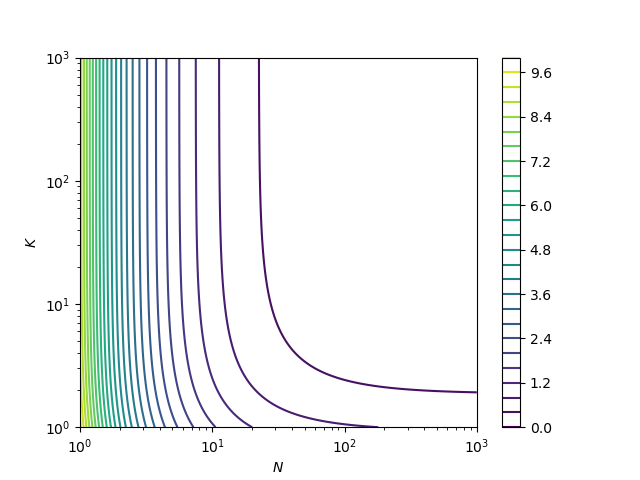
\includegraphics[width=\textwidth]{oigsus_vahe_relatiive_viga_dispersioon.png}  
    \end{center}
    \caption{Õigsuste vahe lähendi relatiivse vea dispersioon juhusliku valimi suuruse $N$ ning märgendatud tingliku $(a_i \neq b_i)$ valimi suuruse $K$ suhtes. Juhul kui $\Delta\accuracy=5\%$ ja $\beta=10\%$. Heledus tähistab dispersiooni.}
    \label{fig:õigsus vahe lähend relatiivne viga dispersioon}
\end{figure}

Jooniselt \ref{fig:õigsus vahe lähend relatiivne viga dispersioon} ning vahetulemuste \eqref{eq:beta relatiivne viga dispersioon} ja \eqref{eq:gamma relatiivne viga dispersioon} kaudu on näha, et $\Delta\widehat{\accuracy}$ relatiivse vea dispersioon kahaneb valimisuuruste kasvades. Telgedel olevatest suurustest tähistab $N$ valimi suurust, mida ei pea märgendama. Kuna sellise valimi leidmine ei ole keeruline võib eeldada, et $N$ on fikseeritud ja küllaltki suur. Oluline on aga suurus $K$, mis tähistab märgendamist vajavate andmepunktide arvu. Märgendatud valimi suuruse prognoosimiseks fikseeritud $N$ põhjal võib uurida olukorda, kus saavutatakse võrdsed lähendite $\hat{\beta}$ ja $\hat{\gamma}$ dispersioonid
\begin{equation}
    \label{eq:võrdsed vahe relatiivse vea dispersioonid}
    \frac{1}{N}\cdot\frac{1-\beta}{\beta}=\frac{1}{K}\cdot(1-\gamma^2) \enspace.
\end{equation}
Kuna $\Delta\accuracy=\beta\cdot\gamma$, on valem \eqref{eq:võrdsed vahe relatiivse vea dispersioonid} esitatav kujul
\begin{equation}    
    K = N \cdot \frac{\beta}{1-\beta} \cdot \left( 1 - \frac{(\Delta\accuracy)^2}{\beta^2} \right) \enspace,
\end{equation}
mille põhjal on võimalik hinnata märgendatud valimi suurust.

\subsection{Saagiste vahe lähendamine}
Saagise puhul on hinnangu \eqref{eq:saagis vahe lähend} analüüsimine keerulisem, kuna saagise definitsioonis on tinglik keskväärtus. Valemile \eqref{eq:õigsus vahe tähistega} analoogi tuletamiseks peab kõigepealt eraldama saagise definitsioonist tingliku jaotuse
\begin{align*}
    \mean{A=Y \mid Y=1}&=\mean{A=1 \mid Y=1}=\prob{A=1 \mid Y=1}\enspace, \\
    \mean{B=Y \mid Y=1}&=\mean{B=1 \mid Y=1}=\prob{B=1 \mid Y=1}\enspace,
\end{align*}
millest saab tuletada
\begin{align*}
    \mean{A=Y \mid Y=1}&=\frac{\prob{A=1 \land Y=1}}{\prob{Y=1}} =\frac{\mean{[A=1]\cdot[Y=1]}}{\mean{Y=1}} \enspace.
\end{align*}
Analoogselt meetodi $B$ puhul
\begin{align*}
    \mean{A=Y \mid Y=1}&=\frac{\prob{B=1 \land Y=1}}{\prob{Y=1}} =\frac{\mean{[B=1]\cdot[Y=1]}}{\mean{Y=1}} \enspace.
\end{align*}
Nende kahe võrduse põhjal võib saagiste vahe esitada kujul
\begin{align*}
    \Delta\recall&=\mean{A=Y \mid Y=1}-\mean{B=Y \mid Y=1} \\
    &=\frac{\mean{[A=1]\cdot[Y=1]-[B=1]\cdot[Y=1]}}{\mean{Y=1}} \enspace.
\end{align*}
Sellest saab järeldada algse saagise lähendi valemi \eqref{eq:saagis lähend} põhjal, et ka saagiste vahe lähend \eqref{eq:saagis vahe lähend} on nihketa. Kuid sellisel kujul esitatud vahele $\Delta\recall$ ei ole lähendi leidmine märgendamise seisukohalt veel kõige parem.

Kehtivad seosed
\begin{align*}
    \mean{[A=1][Y=1]} &= \mean{[A=1][Y=1][B=1]} + \mean{[A=1][Y=1][B=0]} \enspace, \\
    \mean{[B=1][Y=1]} &= \mean{[B=1][Y=1][A=1]} + \mean{[B=1][Y=1][A=0]} \enspace,
\end{align*}
nende seoste ja keskväärtuse definitsiooni põhjal on saagise vahe lugeja esitatav korrutisena tõenäosusest ja tinglikust keskväärtusest
\begin{align*}
    &\mean{[A=1][Y=1]-[B=1][Y=1]} \\
    &=\mean{[A=1][Y=1][A\neq B]-[B=1][Y=1][A\neq B]} \\
    &=\prob{A\neq B}\cdot\mean{[A=1][Y=1]-[B=1][Y=1] \mid [A\neq B]} \enspace.
\end{align*}
Edasiste arvutuste selgemaks esitamiseks on jällegi hea kasutusele võtta tähistused
\begin{align*}
    \beta&=\prob{A\neq B} \enspace, \\
    \nu&=\prob{Y=1} \enspace, \\
    \eta&=\mean{[A=1][Y=1]-[B=1][Y=1] \mid [A\neq B]} \enspace,
\end{align*}
mille kaudu saab esitada saagiste vahe
\begin{equation}
    \label{eq:saagis vahe tähistega}
    \Delta\recall=\frac{\beta\cdot\eta}{\nu} \enspace.
\end{equation}

Tulemuse \eqref{eq:saagis vahe tähistega} põhjal on võimalik meetodite saagiste vahet hinnata lähendades suurusi $\beta$, $\nu$ ja $\eta$. Tõenäosuse $\beta$ puhul on hinnang leitav samamoodi nagu \eqref{eq:beta lähend} eelmises alampeatükis. Ning $\nu$ lähend sarnaselt üle $N$ suuruse juhusliku valimi
\begin{align*}
    \hat{\beta}&=\sum_{i=1}^N [a_i \neq b_i] \enspace, \\
    \hat{\nu}&=\sum_{i=1}^N [y_i = 1] \enspace.
\end{align*}
Tinglikku keskväärtust $\eta$ on võimalik lähendada valimikeskmisena üle tingliku valimi, kus $a_i \neq b_i$. Olgu selle valimi suurus $K$, siis
\begin{equation*}
    \hat{\eta}=\frac{1}{K}\cdot\sum_{i=1}^K [a_i=1][y_i=1]-[b_i=1][y_i=1] \enspace.
\end{equation*}
Kuna hinnangute $\hat{\beta}$ ja $\hat{\nu}$ puhul on summa liikmete võimalikud väärtused $0$ ja $1$, on lähendite absoluutse ja relatiivse vea hinnangud leitavad meetoditega eelmisest peatükist. Kuna lähendi $\hat{\eta}$ puhul on summa liikmete võimalikud väärtused $-1$, $0$, ja $1$, ei saa rakendada binoomjaotusel põhinevaid tulemusi. See-eest on endiselt võimalik kasutada Höffdinig võrratust lähendi absoluutse vea jaoks, seekord tõketega $-1$ ja $1$, mille põhjal avaldub valimi vajalik suurus
\begin{equation*}
    K \geq - \frac{2}{\varepsilon^2} \cdot \ln{\left( \frac{\alpha}{2} \right)} \enspace,
\end{equation*}
kus $\varepsilon$ tähistab absoluutse vea absoluutväärtuse maksimaalset lubatud suurust ning $\alpha$ olulisust.

Relatiivse vea korrutise \eqref{eq:korrutise relatiivne viga dispersioon ligikaudne} ja jagatise \eqref{eq:jagatis relatiivne viga dispersioon} dispersiooni omaduste põhjal võib saagise vahe hinnangu relatiivse vea dispersiooni esitada summana
\begin{equation*}
    \variance{\frac{\hat{\beta}\cdot\hat{\eta}}{\hat{\nu}}:\frac{\beta\cdot\eta}{\nu}}\approx\variance{\frac{\hat{\beta}}{\beta}}+\variance{\frac{\hat{\nu}}{\nu}}+\variance{\frac{\hat{\eta}}{\eta}} \enspace,
\end{equation*}
millest
\begin{equation*}
    \variance{\frac{\hat{\beta}}{\beta}}=\frac{1}{N}\cdot\frac{1-\beta}{\beta},\qquad \variance{\frac{\hat{\nu}}{\nu}}=\frac{1}{N}\cdot\frac{1-\nu}{\nu} \enspace. \\
\end{equation*}
Ning kuna $\eta$ relatiivse vea dispersioon siin kasutusel olevate tähiste kaudu ilusalt ei esitu, võib seda lähendada ka kasutades valimidispersiooni valemit.

\subsection{Täpsuste vahe lähendamine}
Täpsuse jaoks on võrrandi \eqref{eq:saagis vahe tähistega} analoogi tuletamine keeruline, sest täpsuste vahe lähendis on summa liikmed mittesõltumatud. Üheks võimalikuks lahenduseks täpsuse hindamisel on kahesammuline lähenemine, kus hinnatakse esmalt lähendi \eqref{eq:täpsus vahe lähend kole} dispersiooni funktsioonina valikumeetodi abil saadud $S$ elemendilisest valimist (kahe keskmise vahe) ning seejärel lähendatakse selle optimeeritud esitust \eqref{eq:täpsus vahe lähend} veelgi väiksema $K$-elemendilise juhuvalimiga. Kuna saadud lahendus ei ole elegantne ning kõik sammud iseseisvalt on analoogsed peatükis \ref{section:kvaliteedimõõtude veahinnangud} saadud tulemustega, siis ei ole seda antud töös pikemalt käsitletud.
\section{Kokkuvõte}
Töös leiti vajalikud valimi suurused kindluse, veahinnangu lubatud maksimaalse suuruse ja mõnel juhul oletatud tegeliku kvaliteedimõõdu suhtes.Höffdingi võrratuse põhjal leitud tulemused ülehindasid vajaliku valimi suurust võrreldes binoomjaotuse omaduste põhjal arvutatud tulemustega, halvimal juhul isegi suurusjärgu võrra. Tehes arvutusi binoomjaotuse omaduste põhjal, pidi oletama kvaliteedimõõdu tegelikku väärtust. See-eest andis Höffdingi võrratus universaalse hinnangu, mis oli sõltumatu meetodi tegelikust kvaliteedimõõdust (binoomjaotuse parameetrist $p$).

Tehtud töös uuriti ka tehnikaid kahe masinõppe meetodi võrdlemiseks kvaliteedimõõtude põhjal. Uue mudeli kasutusele võtmisel oli küsimuseks kui palju see vanast parem on. Vastust küsimusele otsiti meetodite kvaliteedimõõtude vahede kaudu. Õigsuse ja täpsuse puhul oli võimalik vahele hinnangut leida niimoodi, et manuaalselt peab märgendama vaid andepunkte, mille puhul meetodite klassifikatsioonid erinevad. Selle tulemusel oli võimalik vähendada märgendamist vajavate andmepunktide arvu. Saagise puhul on osa lähendist avaldatav sarnaselt õigsusele ja täpsusele. Kuid saagise arvutamiseks peab ikkagi teadma kõikide andmepunktide tegelikke klassimärgendeid, seega on saagise hindamine märgendamise mõttes ikka raske.

Lisaks uuriti viise kuidas lähendada kvaliteedimõõtude vahesid komponentide kaupa. Definitsioonis kirjeldatud vahe eraldati komponentideks, millest iga komponenti oli võimalik lähendada erinevate valimitega kasutades tulemusi eelnevatest peatükkidest. Tulemusena oli osa vahe hinnangust leitav täiesti märgendamata valimil. Saagise olemuse tõttu oli saagise hindamine märgendamise seisukohalt ikka kulukas.

% viited
\newpage
\printbibliography[title={Viidatud kirjandus}]

% lisad
\section*{Lisad}
\selectlanguage{estonian}

\section*{I. Lähtekood}
Töös esitatud graafikute lähtekood on kättesaadaval aadressil \url{https://github.com/mart-mihkel/mudelite_hindamine}.

\newpage
\section*{II. Litsents}
\subsection*{Lihtlitsents lõputöö reprodutseerimiseks ja üldsusele kättesaadavaks tegemiseks}
Mina, \textbf{Mart-Mihkel Aun}, 
\begin{enumerate}
    \item
    annan Tartu Ülikoolile tasuta loa (lihtlitsentsi) minu loodud teose
    \par
    \textbf{Masinõppe mudelite hindamine väheste märgenditega andmetel}
    \par
    mille juhendaja on Sven Laur,
    \par
    reprodutseerimiseks eesmärgiga seda säilitada, sealhulgas lisada digitaalarhiivi DSpace kuni autoriõiguse kehtivuse lõppemiseni.
    \par
    \item

    Annan Tartu Ülikoolile loa teha punktis 1 nimetatud teos üldsusele kättesaadavaks Tartu Ülikooli veebikeskkonna, sealhulgas digitaalarhiivi DSpace kaudu Creative Commonsi litsentsiga CC BY NC ND 3.0, mis lubab autorile viidates teost reprodutseerida, levitada ja üldsusele suunata ning keelab luua tuletatud teost ja kasutada teost ärieesmärgil, kuni autoriõiguse kehtivuse lõppemiseni.
    \item
    Olen teadlik, et punktides 1 ja 2 nimetatud õigused jäävad alles ka autorile.
    \item
    Kinnitan, et lihtlitsentsi andmisega ei riku ma teiste isikute intellektuaalomandi ega isikuandmete kaitse õigusaktidest tulenevaid õigusi. 
\end{enumerate}
\noindent
Mart-Mihkel Aun\\
\textbf{\textsl{09.05.2023}}

\end{document}